\chapter{Modelagem matemática }

\section{Modelagem matemática}

Dentro da pesquisa, foram realizadas duas modelagens distintas, ambas, diferentemente da literatura clássica, foram elaboradas com base nas estações de origem e destino, e não nos legs do percurso.

Para compreender essas propostas, consideremos uma versão simplificada do problema como se mostra na figura \ref{fig: fig1}, onde temos:

\begin{itemize}
	\item 4 estações pelas quais o trem deve passar em um único sentido, ou seja, o trem não tem retorno.
	\item O trem tem uma capacidade física máxima de assentos.
	\item Há apenas um tipo de classe comercial.
	\item Existe apenas um período no horizonte de reserva.
	\item A variável de decisão é a quantidade de assentos que pode ser disponibilizada para venda em um trecho com origem e destino específicos.
	\item Todos os assentos disponibilizados para venda serão vendidos.
\end{itemize}

\begin{figure}[th]
	\begin{center}
		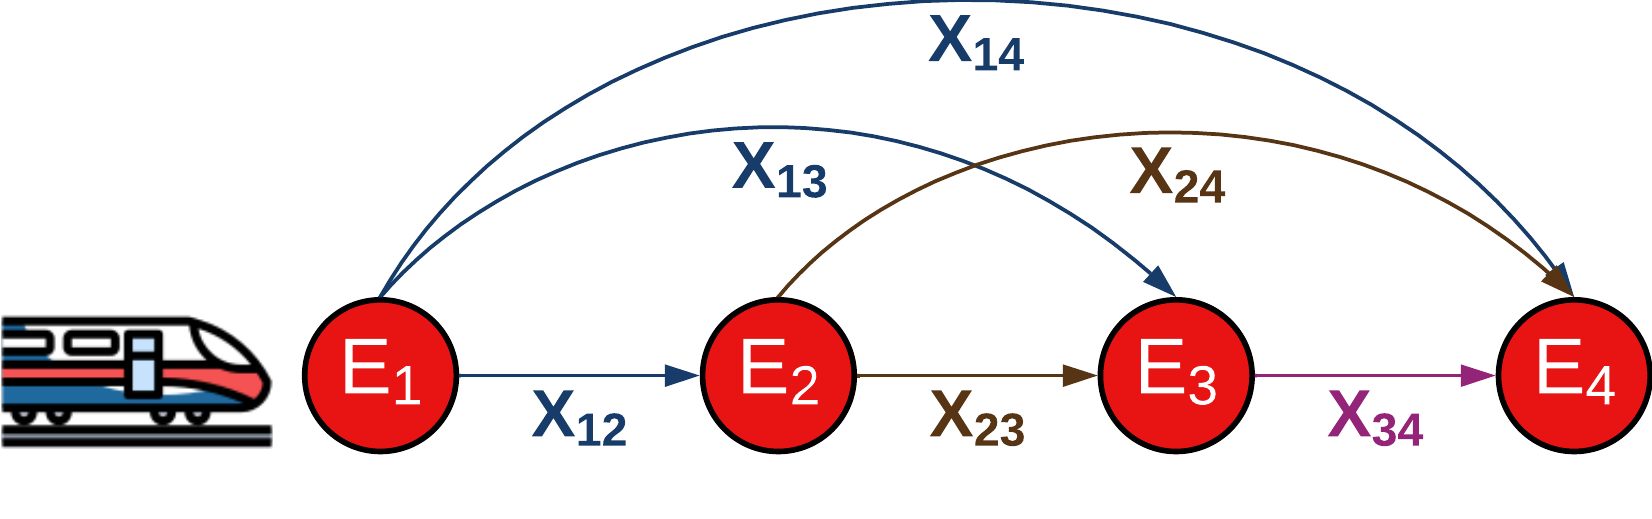
\includegraphics[scale=0.18]{img/repre_ini1.png}
		\caption{Versão gráfica simples do Problema de Transporte Ferroviário de Passageiros}
		% Fonte:~\cite{khaksar2013genetic}}
		\label{fig: fig1}
	\end{center}
\end{figure}


\section{Primeira modelagem: Demanda Independente}\label{sec:modelo1}

Para este modelo, assumiremos uma demanda independente, o que significa que cada cliente pode comprar um produto específico independentemente da oferta disponível no momento da compra. Em outras palavras, pode-se dizer que, se um cliente estiver disposto a pagar um valor, por exemplo, de 10 reais por um assento, ele comprará o bilhete exatamente por esse valor, mesmo que um preço mais baixo esteja disponível. Agora, se o cliente não encontrar esse valor exato, ele preferirá não comprar.

Então, para esta proposta, temos o seguinte

\noindent $x_{ij}$: Quantidade de assentos que serão reservados no trecho com origem em $i$ e destino em $j$, onde $j>i$ (variável de decisão). \\
\noindent $A_i$: Quantidade de assentos vagos na estação $i$. \\
\noindent $P_{ij}$: Preço da passagem no trajeto com origem em $i$ e destino em $j$. \\
\noindent $Q$: Capacidade física do trem.

Dado o exposto, a função objetivo será maximizar o lucro para cada possível venda em cada trajeto $i,j$, matematicamente seria:

$FO: max \quad x_{12}P_{12} + x_{13}P_{13} + x_{14}P_{14} + x_{23}P_{23} + x_{24}P_{24} + x_{34}P_{34}$

s.a.

Estação 1: $x_{12} + x_{13} + x_{14} \leq A_1 \quad onde \quad A_1 = Q $ \\
\indent Estação 2: $x_{23} + x_{24}  \leq  A_2 \quad onde \quad A_2 = A_1 - (x_{12} + x_{13} + x_{14}) + x_{12} $ \\
\indent Estação 3: $x_{34} \leq A_3 \quad onde \quad A_3 = A_2 - (x_{23} + x_{24}) + x_{13} + x_{23} $

Note que as restrições são aplicadas para cada uma das três primeiras estações, $E_1, E_2$ e $E_3$, já que são as estações que têm pelo menos um destino, e a última estação, E4, é excluída, pois não possui nenhum destino.

Cada uma das restrições leva em consideração o fluxo de pessoas que sairão e entrarão no trem. Levando isso em conta, é necessário calcular a disponibilidade do trem para cada estação. Considere uma solução viável para o modelo, conforme mostrado na figura \ref{fig: fig2}, com uma capacidade total de 100 assentos para um trem.

\begin{figure}[!ht]
	\begin{center}
		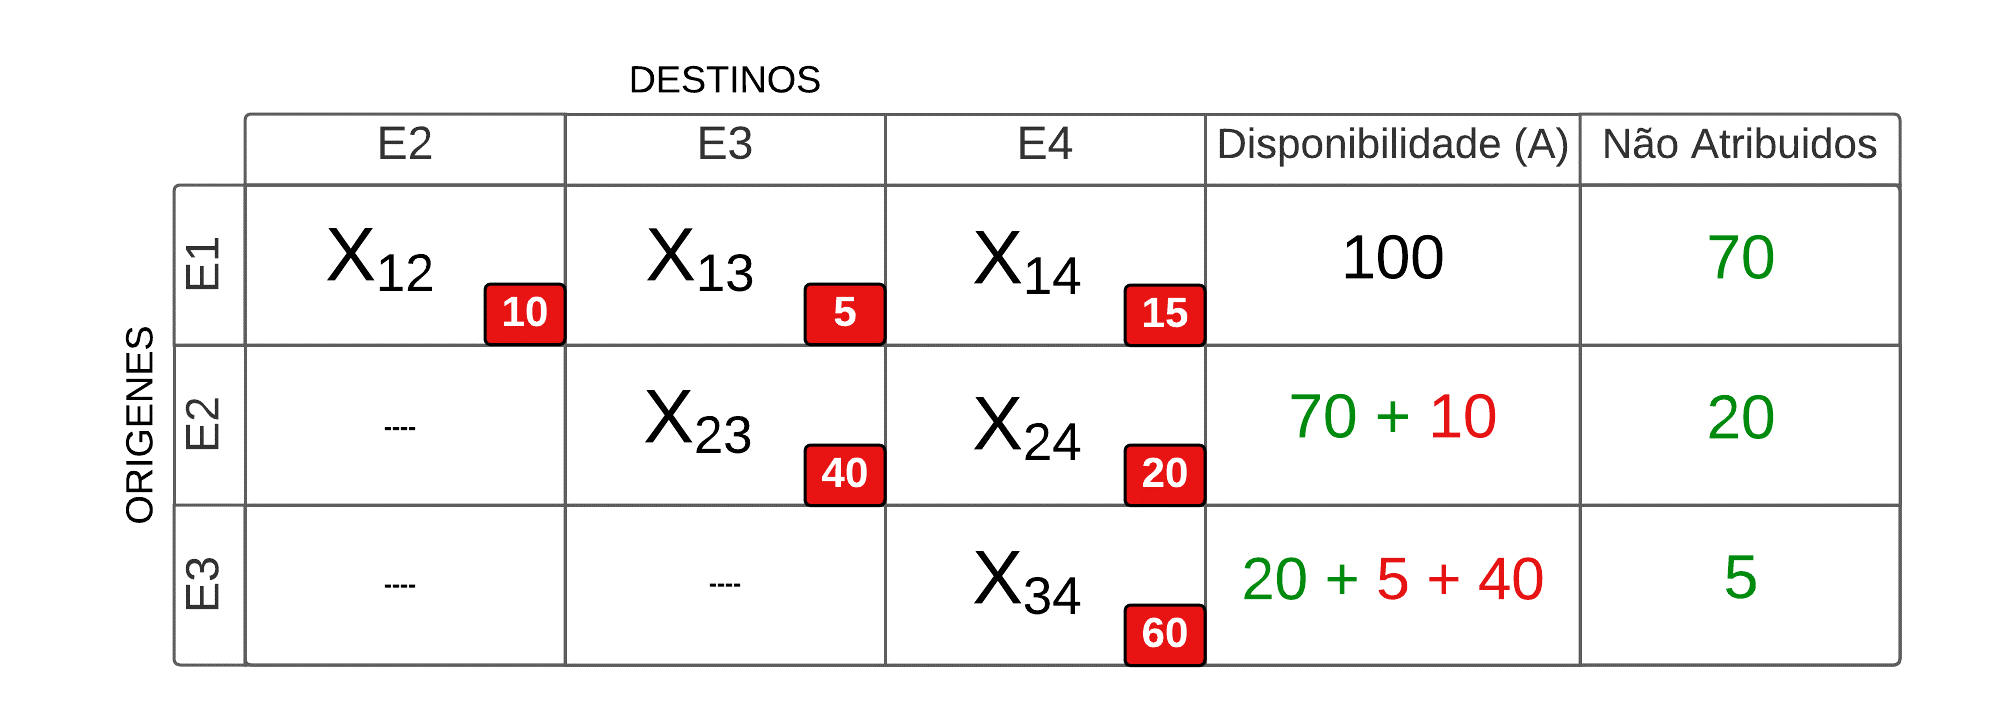
\includegraphics[scale=0.4]{img/fig2.png}
		\caption{Solução factível para o problema simplificado}
		% Fonte:~\cite{khaksar2013genetic}}
		\label{fig: fig2}
	\end{center}
\end{figure}

Note que, para a restrição da estação 1, o trem está com todos os assentos vazios, ou seja, \(A_1=100\), e que a soma das variáveis seria \(x_{12} + x_{13} + x_{14} = 10 + 5 + 15 = 30\). Portanto, teríamos \(30 \leq 100\), ou seja, foram disponibilizados para venda 30 assentos dos 100 que o trem possui. Nesse sentido, no momento da partida do trem da estação 1, haveria 70 assentos vazios ou disponíveis para venda em estações posteriores.

Agora, para a estação 2, teríamos \(A_2 = 100 - 30 + 10 = 70 + 10 = 80\). Já era conhecido que havia 70 assentos disponíveis vindos da estação 1, mas também é preciso levar em conta que os assentos com destino à estação 2 também ficarão disponíveis da estação 2 em diante, para este caso \(x_{12} = 10\). Portanto, para a estação 2, teríamos 80 assentos vazios para disponibilizar, ou seja, \(60 \leq 80\). Analogamente, o mesmo raciocínio seria aplicado para a estação 3, ou seja, teríamos a soma de todos os assentos que chegaram à estação 3, \(x_{13} = 5\) e \(x_{23} = 40\), assim teríamos \(A_3 = 80 - 60 + 5 + 40 = 20 + 5 + 40 = 65\), e no final teríamos \(60 \leq 65\).

Além da lógica anterior, assume-se que há um trem, com vários tipo de assento, que viajará de uma estação $E_1$ até uma estação $E_n$ (onde $n$ é a última estação onde o trem chegará). Esse trem terá um itinerário que conterá o nome do trem, a estação de origem, a estação de destino, a data e hora de partida e de chegada. Além disso, haverá uma lista de preços (para cada tipo de assento) a ser disponibilizada para venda. Cada um dos preços da lista será chamado de classe de controle ou control class. Os bilhetes serão disponibilizados para venda antes da partida do trem, e o tempo entre a disponibilização e a referida partida será chamado de horizonte de reserva. Esse horizonte será dividido em vários períodos, que podem ter diferentes temporalidades. Por exemplo, pode haver períodos em dias, semanas, meses, etc., e combinações entre eles. Os períodos dentro do horizonte de reserva estão ordenados de forma descendente, onde o menor valor é zero e representa a data de partida do trem, e o valor maior representa a data de disponibilização das vendas, $[ t,t-1,t-2,...,0]$.

Cada relação possível entre uma estação e outra será denominada origem-destino ou trecho. Será dito que uma origem-destino é adjacente se, e somente se, não houver estações intermediárias entre elas; caso contrário, serão não adjacentes. Por exemplo, na figura \ref{fig: fig1}, os trechos adjacentes seriam: $(E_1-E_2)$, $(E_2-E_3)$, $(E_3-E_4)$, e os trechos não adjacentes seriam: $(E_1-E_3)$, $(E_1-E_4)$ e $(E_2-E_4)$. Além disso, observe que os trechos não adjacentes podem conter outros trechos, tanto adjacentes quanto não adjacentes. Por exemplo, o trecho $(E_1-E_4)$ da figura \ref{fig: fig1} contém os trechos adjacentes $(E_1-E_2)$, $(E_2-E_3)$, e contém os trechos não adjacentes $(E_1-E_3)$ e $(E_2-E_4)$. Vejamos o modelo completo:


% Vejamos agora o modelo proposto completo:
\begin{table}[H]
	\centering
	\small
	\begin{tabular}{p{2cm} p{9.5cm} p{3.2cm}}
		\toprule
		\textbf{Definição} & \textbf{Descrição}                                                                                                                                                                                                                                                                                                                                                                                                            & \textbf{Domínio}                             \\ \midrule
		\multicolumn{3}{l}{\textbf{Conjuntos}}                                                                                                                                                                                                                                                                                                                                                                                                                                                            \\ \midrule
		$O$                & Conjunto de Estações de origem                                                                                                                                                                                                                                                                                                                                                                                                &                                              \\
		$D$                & Conjunto de Estações de Destino                                                                                                                                                                                                                                                                                                                                                                                               &                                              \\
		$OD$               & Conjunto de Trechos com itinerário                                                                                                                                                                                                                                                                                                                                                                                            &                                              \\
		$NAD$              & \multicolumn{2}{p{12.7cm}}{Conjunto de Trechos que NÃO são Adjacentes e que tem itinerário}                                                                                                                                                                                                                                                                                                                                                                                  \\
		$BRI_{(o,d)}$      & \multicolumn{2}{p{12.7cm}}{Conjunto de Trechos contidos dentro de cada trecho $(o,d)$ NÃO Adjacente }                                                                                                                                                                                                                                                                                                                                                                        \\
		$CR_{(o,d)}$       & \multicolumn{2}{p{12.7cm}}{É um conjunto que contém outros subconjuntos, onde cada subconjunto é uma rota possível para ir desde a origem $o$ até o destino $d$, sendo $(o,d)$ não adjacente. Por exemplo, para a rota $E_1 - E_4$ da figura \ref{fig: fig1}, $CR_{(E_1,E_4)}=\{ \textcolor{green}{\{} (E_1-E_2),(E_2-E_4)\textcolor{green}{\}}, \textcolor{blue}{\{} (E_1-E_3),(E_3-E_4)\textcolor{blue}{\}}, \textcolor{red}{\{}(E_1-E_2),(E_2-E_3),(E_3-E_4) \textcolor{red}{\}} \} $}                                                                                                                                                                                                                                 \\
		$S$                & Representa cada subconjunto dentro de $CR_{(o,d)}$                                                                                                                                                                                                                                                                                                                                                                          &                                              \\
		$V$                & Conjunto de tipos de assento do trem                                                                                                                                                                                                                                                                                                                                                                                                 &                                              \\
		$T$                & Conjunto de Períodos                                                                                                                                                                                                                                                                                                                                                                                           &                                              \\
		$K_v$              & \multicolumn{2}{p{12.7cm}}{É o conjunto de classes de controle para cada tipo de assento $v$. Por exemplo, suponha que há dois tipos de assento $z$ e $p$, e cada tipo contém três classes de controle $c_1, c_2, c_3$, então a representação seria $K_z:\{c_1,c_2,c_3\}$ e $K_p:\{c_1,c_2,c_3\}$. Além disso, considere que os elementos de cada $K_v$ são ordenados, onde sempre se cumpre que a classe de menor índice é a classe mais custosa, ou seja $c_1>c_2>c_3$.}                    \\ \midrule
		\multicolumn{3}{l}{\textbf{Parâmetros}}                                                                                                                                                                                                                                                                                                                                                                                                                                                           \\ \midrule
		$n$                & Quantidade de Estações                                                                                                                                                                                                                                                                                                                                                                                                        &                                              \\
		$Q_v$              & Capacidade física do trem para cada tipo de assento $v$                                                                                                                                                                                                                                                                                                                                                                         & $v \in V$                                    \\
		$P_{ijvk}$         & Preços  das passagens no Trecho $(i,j)$, tipo de assento $v$ e Classe de Control $k$                                                                                                                                                                                                                                                                                                                                                    & $(i,j) \in OD,v \in V, k \in K_v$            \\
		$d_{ijvkt}$        & Demanda Independente no Trecho $(i,j)$, tipo de assento $v$ e Classe de Control $k$                                                                                                                                                                                                                                                                                                                                                   & $(i,j) \in OD,v \in V, k \in K_v, t \in T$   \\ \midrule
		% $d'_{ijvkt}$       & Demanda Comportamental no Trecho $(i,j)$, tipo de assento $v$ e Classe de Control $k$                                                                                                                                                                                                                                                                                                                                                  & $(i,j) \in OD,v \in V, k \in K_v, t \in T$   \\ 
		% \multicolumn{3}{l}{\textbf{Variáveis de decisão}}                                                                                                                                                                                                                                                                                                                                                                                                                                                 \\ \midrule
		% $X_{ijvkt}$        & Quantidade de passagens reservadas no trecho $(i,j)$, tipo de assento $v$ e com classe de control $k$ no período $t$                                                                                                                                                                                                                                                                                                                    & $(i,j) \in OD, v \in V, k \in K_v, t \in T$  \\
		% $Y_{ijvkt}$        & Quantidade de passagens autorizados no trecho $(i,j)$, tipo de assento $v$ e com classe de control $k$ no período $t$                                                                                                                                                                                                                                                                                                                   & $(i,j) \in OD, v \in V, k \in K_v, t \in T$  \\
		% $\gamma_{ijvkt}$       & É uma variavel binaria que toma o valor de 1 quando $Y_{ijvkt} \neq 0$ e toma  valor de 0 caso contrario                                                                                                                                                                                                                                                                                                                      & $(i,j) \in OD, v \in V, k \in K_v, t \in T$ \\
		% $\beta_{ijvkt}$       & É uma variavel binaria que toma o valor de 1 quando a classe $k$ é a classe mais barata que foi autorizada para venda, no trecho $i,j$, tipo de assento $v$ e periodo $t$; e toma  valor de 0 caso contrario                                                                                                                                                                                                                                                                    & $(i,j) \in OD, v \in V, k \in K_v, t \in T$  \\
		% $\alpha_{ijvkt}$       & É uma variavel binaria que toma o valor de 1 quando $X_{ijvkt} \neq 0$ e toma  valor de 0 caso contrario                                                                                                                                                                                                                                                                                                                      & $(i,j) \in OD, v \in V, k \in K_v, t \in T$ \\
		% \multicolumn{3}{l}{\textbf{Variável auxiliar}}                                                                                                                                                                                                                                                                                                                                                                                                                                                    \\ \midrule
		% $A_{iv}$            & Armazena a quantidade de assentos vazios disponíveis para venda em cada estação de origem e cada tipo de assento durante todo o horizonte de reserva. Cabe esclarecer que esta não é uma variável de decisão, pois esta variável apenas armazena um cálculo com base na capacidade física do trem e nas variáveis de decisão de passagens reservadas                                                                                                          & $i \in O, v \in V$                                    \\
		% \bottomrule
	\end{tabular}
	\caption{Notação matemática do problema}
	\label{tab: m1_definicao1}
\end{table}


% Vejamos agora o modelo proposto completo:
\begin{table}[H]
	\centering
	\small
	\begin{tabular}{p{2cm} p{9.5cm} p{3.2cm}}
		\toprule
		\textbf{Definição} & \textbf{Descrição}                                                                                                                                                                                                                                                                                                                                                                                                            & \textbf{Domínio}                             \\ \midrule
		% \multicolumn{3}{l}{\textbf{Conjuntos}}                                                                                                                                                                                                                                                                                                                                                                                                                                                            \\ \midrule
		% $O$                & Conjunto de Estações de origem                                                                                                                                                                                                                                                                                                                                                                                                &                                              \\
		% $D$                & Conjunto de Estações de Destino                                                                                                                                                                                                                                                                                                                                                                                               &                                              \\
		% $OD$               & Conjunto de Trechos com itinerário                                                                                                                                                                                                                                                                                                                                                                                            &                                              \\
		% $NAD$              & \multicolumn{2}{p{12.7cm}}{Conjunto de Trechos que NÃO são Adjacentes e que tem itinerário}                                                                                                                                                                                                                                                                                                                                                                                  \\
		% $BRI_{(o,d)}$      & \multicolumn{2}{p{12.7cm}}{Conjunto de Trechos contidos dentro de cada trecho $(o,d)$ NÃO Adjacente }                                                                                                                                                                                                                                                                                                                                                                        \\
		% $CR_{(o,d)}$       & \multicolumn{2}{p{12.7cm}}{É um conjunto que contém outros subconjuntos, onde cada subconjunto é uma rota possível para ir desde a origem $o$ até o destino $d$, sendo $(o,d)$ não adjacente. Por exemplo, para a rota $E_1 - E_4$ da figura \ref{fig: fig1}, $CR_{(E_1,E_4)}=\{ \textcolor{green}{\{} (E_1-E_2),(E_2-E_4)\textcolor{green}{\}}, \textcolor{blue}{\{} (E_1-E_3),(E_3-E_4)\textcolor{blue}{\}}, \textcolor{red}{\{}(E_1-E_2),(E_2-E_3),(E_3-E_4) \textcolor{red}{\}} \} $}                                                                                                                                                                                                                                 \\
		% $S$                & Representa cada subconjunto dentro de $CR_{(o,d)}$                                                                                                                                                                                                                                                                                                                                                                          &                                              \\
		% $V$                & Conjunto de tipo de assento do trem                                                                                                                                                                                                                                                                                                                                                                                                   &                                              \\
		% $T$                & Conjunto de Check-Points (Períodos)                                                                                                                                                                                                                                                                                                                                                                                           &                                              \\
		% $K_v$              & \multicolumn{2}{p{12.7cm}}{É o conjunto de classes de controle para cada tipo de assento $v$. Por exemplo, suponha que há dois tipo de assento, $z$ e $p$, e cada tipo de assento contém três classes de controle $c_1, c_2, c_3$, então a representação seria $K_z:\{c_1,c_2,c_3\}$ e $K_p:\{c_1,c_2,c_3\}$. Além disso, considere que os elementos de cada $K_v$ são ordenados, onde sempre se cumpre que a classe de menor indice é a classe mais costosa, ou seja $c_1>c_2>c_3$.}                    \\ \midrule
		% \multicolumn{3}{l}{\textbf{Parâmetros}}                                                                                                                                                                                                                                                                                                                                                                                                                                                           \\ \midrule
		% $n$                & Quantidade de Estações                                                                                                                                                                                                                                                                                                                                                                                                        &                                              \\
		% $Q_v$              & Capacidade física do trem para cada tipo de assento $v$                                                                                                                                                                                                                                                                                                                                                                         & $v \in V$                                    \\
		% $P_{ijvk}$         & Preços  das passagens no Trecho $(i,j)$, tipo de assento $v$ e Classe de Control $k$                                                                                                                                                                                                                                                                                                                                                    & $(i,j) \in OD,v \in V, k \in K_v$            \\
		% $d_{ijvkt}$        & Demanda Independente no Trecho $(i,j)$, tipo de assento $v$ e Classe de Control $k$                                                                                                                                                                                                                                                                                                                                                   & $(i,j) \in OD,v \in V, k \in K_v, t \in T$   \\ \midrule
		\multicolumn{3}{l}{\textbf{Variáveis de decisão}}                                                                                                                                                                                                                                                                                                                                                                                                                                                 \\ \midrule
		$X_{ijvkt}$        & Quantidade de passagens reservadas no trecho $(i,j)$, tipo de assento $v$ e com classe de control $k$ no período $t$                                                                                                                                                                                                                                                                                                                    & $(i,j) \in OD, v \in V, k \in K_v, t \in T$  \\
		$Y_{ijvkt}$        & Quantidade de passagens autorizados no trecho $(i,j)$, tipo de assento $v$ e com classe de control $k$ no período $t$                                                                                                                                                                                                                                                                                                                   & $(i,j) \in OD, v \in V, k \in K_v, t \in T$  \\
		$\gamma_{ijvkt}$       & É uma variável binaria que toma o valor de 1 quando $Y_{ijvkt} \neq 0$ e toma  valor de 0 caso contrario                                                                                                                                                                                                                                                                                                                      & $(i,j) \in OD, v \in V, k \in K_v, t \in T$ \\
		$\beta_{ijvkt}$       & É uma variável binaria que toma o valor de 1 quando a classe $k$ é a classe mais barata que foi autorizada para venda, no trecho $i,j$, tipo de assento $v$ e período $t$; e toma  valor de 0 caso contrario                                                                                                                                                                                                                                                                    & $(i,j) \in OD, v \in V, k \in K_v, t \in T$  \\
		$\alpha_{ijvkt}$       & É uma variável binaria que toma o valor de 1 quando $X_{ijvkt} \neq 0$ e toma  valor de 0 caso contrario                                                                                                                                                                                                                                                                                                                      & $(i,j) \in OD, v \in V, k \in K_v, t \in T$ \\
		\multicolumn{3}{l}{\textbf{Variável auxiliar}}                                                                                                                                                                                                                                                                                                                                                                                                                                                    \\ \midrule
		$A_{iv}$            & Armazena a quantidade de assentos vazios disponíveis para venda em cada estação de origem e cada tipo de assento durante todo o horizonte de reserva. Cabe esclarecer que esta não é uma variável de decisão, pois esta variável apenas armazena um cálculo com base na capacidade física do trem e nas variáveis de decisão de passagens reservadas                                                                                                          & $i \in O, v \in V$                                    \\
		\bottomrule
	\end{tabular}
	\caption{Notação matemática do problema}
	\label{tab: m1_definicao2}
\end{table}

\allowdisplaybreaks
\begin{align}
	 & Max \quad Z = \sum_{(i,j)\in OD} \sum_{v\in V} \sum_{k\in K_v} \sum_{t\in T} P_{ijvk} X_{ijvkt}                                                                                                                \label{eq: m1_fo}                                                             \\
	 & \text{s.a.}  \notag                                                                                                                                                                                                                                                                          \\
	 & A_{iv} = A_{i-1,v} - \sum_{(i,j) \in OD/j \geq i} \sum_{k\in K_v}\sum_{t\in T}X_{i-1,j,v,k,t} + \sum_{(i,j) \in OD/j<i} \sum_{k\in K_v}\sum_{t\in T}X_{jivkt}, \quad \forall i \in O, v \in V  \label{eq: m1_disponi}                                                         \\
	 & \sum_{(i,j) \in OD} \sum_{k\in K_v}\sum_{t\in T} X_{ijvkt} \leq A_{iv} , \quad \forall i \in O /i<j, i < n, v \in V                                                                                       \label{eq: m1_cap_assig}                                                       \\
	%  & \textcolor{red}{ Y_{ijvkt} \geq Y_{i,j,v,k+1,t},  \quad \forall (i,j) \in OD / i < j, v \in V, k \in K_v / k < \lVert K_v \rVert , t \in T }                                                                  \label{eq: m1_jerar_class}                                                     \\   % P_{ijvk} \geq P_{i,j,v,k+1}
	 & \sum_{(i,j) \in OD}\sum_{v\in V}\sum_{t\in T} Y_{i,j,v,k,t} \leq Q_v, \quad  k = min\{K_v\}, \forall i \in O                                                                                                    \label{eq: m1_cap_autho_1er_class}                                             \\
	 & Y_{ijvkt} \geq  X_{ijvkt},  \quad k = max\{K_v\}, \forall(i,j) \in OD ,v \in V, t \in T                                                                                                                       \label{eq: m1_autho_mayor_assig_1er_class}                                     \\
	 & Y_{ijvkt} \geq  X_{ijvkt} + Y_{i,j,v,k + 1,t} , \quad \forall(i,j) \in OD, v \in V, k \in K_v / k < \lVert K_v \rVert , t \in T                                                                               \label{eq: m1_autho_mayor_assig_mas_autho}                                     \\
	 & \textit{\underline{Demanda Independente  }}         \notag                                                                                                                                                                                                                                 \\
	 & \textcolor{red}{X_{ijvkt} \leq d_{ijvkt},  \quad \forall (i,j) \in OD / i < j  ,v \in V, k \in K_v, t\in T }                                                                                                 \label{eq: m1_assig_menor_dem}                                                 \\
	%  & \sum_{k' \in K_v / k' \leq k}X_{i,j,v,k',t} \leq d'_{ijvkt} \quad \forall (i,j) \in OD, v \in V, k \in K_v / k > 1, t\in T                                                                                    \label{eq: m1_dem_compor_acumulacao_class}                                                 \\
	%  & X_{ijvkt} \leq \left( d'_{ijvkt} \right) \left(\frac{d_{ijvkt}}{d'_{i,j,v,k',t}}\right),  \quad \forall (i,j) \in OD, v \in V, k \in K_v/ k < k', k' < max\{K_v\}, t\in T                                     \label{eq: m1_dem_compor_porcentaje_dem}                                                                               \\
	% \begin{split}
	% 	 & X_{i,j,v,k',t} \leq d_{i,j,v,k',t} + \left( d'_{i,j,v,k',t} - \sum_{k \in K_v }\frac{d'_{ijvkt} d_{ijvkt}}{d'_{i,j,v,k',t}} \right),  \quad \forall (i,j) \in OD                                                                                                                         \\
	% 	 & v \in V, k' = max\{K_v\}, t\in T                                                                                                                                                                                                                                                     \\
	% \end{split}                                                                                                                                                                                                      \label{eq: m1_dem_compor_porcentaje_dem_last}                                                                                \\
	 & \textit{\underline{Fulfillments over periods} }   \notag                                                                                                                                                                                                                                    \\
	 & \gamma_{ijvkt} \leq Y_{ijvkt} \leq \gamma_{ijvkt} Q_v, \quad  \forall (i,j)\in OD, v \in V, k \in K_v, t \in T                                                                                                       \label{eq: m1_activ_bin_autho}                                                 \\
	 & \alpha_{ijvkt} \leq X_{ijvkt} \leq \alpha_{ijvkt}d_{ijvkt}, \quad   \forall(i,j) \in OD, v \in V, k \in K_v, t \in T                                                                                                  \label{eq: m1_binaria_alpha}                                                                               \\
	 & \alpha_{ijvkt} \leq \alpha_{i,j,v,k,t+1}, \quad   \forall(i,j) \in OD, v \in V, k \in K_v, t \in T/ t \neq max\{T\}                                                                                                   \label{eq: m1_assig_last_periodo}                                                                              \\
	 & \sum_{k \in K_v}\beta_{ijvkt}P_{ijvk} \geq \sum_{k \in K_v}\beta_{i,j,v,k,t+1}P_{ijvk},  , \quad   \forall(i,j) \in OD, v \in V, t \in T/ t \neq max\{T\}                                                              \label{eq: m1_fulfill_periodo}                          \\
	 & \textit{\underline{Skip Lagging}}    \notag                                                                                                                                                                                                                                                  \\
	 & \beta_{ijvkt} = \gamma_{ijvkt} - \gamma_{i,j,v,k+1,t}, \quad \forall (i,j) \in OD, v \in V, k \in K /k < max\{K_v\}, t\in T                                                                                               \label{eq: m1_binaria_Beta}             \\                                                                   
	 & \beta_{ijvkt} = \gamma_{ijvkt}, \quad   \forall(i,j) \in OD, v \in V, k = max\{K_v\}, t \in T                                                                                                                         \label{eq: m1_binaria_Beta_last}                                                                           \\
	 & \sum_{k \in K_v}\beta_{ijvkt}P_{ijvk} \leq \sum_{k \in K_v}\beta_{i,j',v,k,t}P_{ijvk}, \quad \forall i \in O, j \in D, j' \in D / j' > j, v \in V, t \in T                                                           \label{eq: m1_preco_estacao_inicio}                                                                              \\
	 \begin{split}
	 	& \sum_{k \in K_v}\beta_{odvkt}P_{odvk} \leq \sum_{(i,j) \in S}\sum_{k \in K_v}\beta_{ijvkt}P_{ijvk}, \quad    \forall (o,d) \in NAD, \\
		& v \in V, t \in T , \quad  \forall S \in CR_{o,d} / S \subset CR_{o,d}           \\
	\end{split}                                                                                                                                                                                                       \label{eq: m1_preco_combinacao_rotas_contidas}                                          \\
	 & \textit{\underline{Inicialização e domínio }}    \notag                                                                                                                                                                                                                                      \\
	 & A_{0,v} = Q_v,     \quad  \forall v \in V                                                                                                                                                                                                 \label{eq: m1_ini_disponi}                                                    \\
	 & X_{0,j,v,k,t} = 0,     \quad \forall j \in D, v \in V, k \in K_v, t \in T                                                                                                                                      \label{eq: m1_ini_assig}                                                      \\
	 & X_{ijvkt} \in \mathbb{Z}^+ , \quad   \forall(i,j) \in OD, v \in V, k \in K_v, t \in T                                                                                                                                                                                     \label{eq: m1_dom_assig}                                                      \\
	 & Y_{ijvkt} \in \mathbb{Z}^+ , \quad   \forall(i,j) \in OD, v \in V, k \in K_v, t \in T                                                                                                                                                                                   \label{eq: m1_dom_autho}                                                      \\
	 & A_{iv} \in \mathbb{Z}^+  , \quad \forall i \in O, v \in V                                                                                                                                                                               \label{eq: m1_dom_disponi}                                                    \\
	 & \gamma_{ijvkt}, \beta_{ijvkt}, \alpha_{ijvkt}\in \{0,1\} , \quad   \forall(i,j) \in OD, v \in V, k \in K_v, t \in T                                                                                                                                                                                       \label{eq: m1_dom_bin_nadja}
\end{align}


Na equação \ref{eq: m1_fo}, a qual representa a função objetivo, temos a soma do produto entre a quantidade de assentos reservados a cada trajeto de origem e destino para a classe comercial em cada período e cada tipo de assento, multiplicada pelo preço correspondente para cada trajeto e classe. Observe que queremos maximizar os ingressos em função dos assentos que estão reservados, que é o mais próximo que se tem da realidade em função da demanda conhecida.

A restrição \ref{eq: m1_disponi} é responsável por calcular a quantidade de assentos vazios disponíveis em cada estação de origem, para cada tipo de assento, ao longo de todo o horizonte de reserva. Ela é uma generalização do exemplo simplificado utilizado para calcular $A_{iv}$.

A restrição \ref{eq: m1_cap_assig} garante que os assentos reservados ao longo de todo o horizonte de reserva, para cada trecho, não excedam a capacidade disponível para cada tipo de assento em cada estação de origem.

A restrição \ref{eq: m1_cap_autho_1er_class} garanta que a soma de autorizações da classe mais custosa, de cada estação de origem, de todos os períodos, não ultrapasse a capacidade do trem de cada tipo de assento. Note que apenas estamos considerando a classe mais cara devido à natureza cumulativa das variáveis de autorização é por isso que o valor de k é o mínimo das classes de cada tipo de assento, pois a ordem do nome das classes é crescente mas o seu valor é decrescente. Para melhor compreensão, suponhamos uma solução para um problema de dois vagões $V_1$ e $V_2$, 3 classes para $V_1$ e 3 classes para $V_2$, 5 estações,  10 trechos, um período e uma capacidade física do trem de 700 cadeiras, conforme mostra a figura \ref{fig: autorization}.

\begin{figure}[!ht]
	\begin{center}
		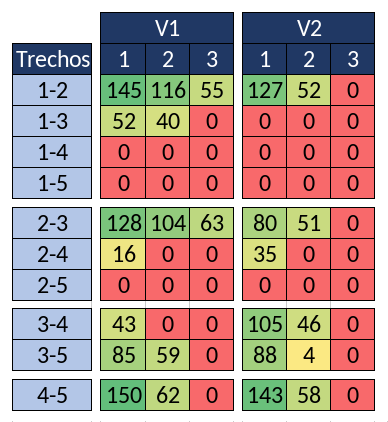
\includegraphics[scale=0.40]{img/exemplo1.png}
		\caption{Solução factível para a variável de decisão Autorização}
		% Fonte:~\cite{khaksar2013genetic}}
		\label{fig: autorization}
	\end{center}
\end{figure}

Observe que os nomes das classes são números ordenados de forma crescente [1, 2, 3] também o valor da classe 1 é mais caro que o valor da classe 2 e este é maior que o valor da classe 3. Além disso, a soma que não ultrapassará a capacidade do trem é a soma das classes 1 de cada tipo de assento de cada estação de origem. Por exemplo, para a estação 3 seria $43 + 85$ para $V_1$ trecho 3-4 e 3-5, mais, $105 + 88$ para $V_2$ nos mesmos trechos, ou seja $43 + 85 + 105 + 88 = 321 \leq 700$


Até ao momento foi referido que a variável $Y$ tem um carácter cumulativo e são as restrições \ref{eq: m1_autho_mayor_assig_1er_class} e \ref{eq: m1_autho_mayor_assig_mas_autho} que controlam este comportamento. A restrição \ref{eq: m1_autho_mayor_assig_1er_class} é um caso particular da restrição \ref{eq: m1_autho_mayor_assig_mas_autho}, aplicada apenas à última classe, ou classe mais barata reservada para cada tipo de assento ($k=max\{K_v\}$), e garante que a soma de todos os períodos, de cada estação de origem da classe mais barata da variável "autorização" é maior ou igual à variável de decisão "reservas" nas mesmas condições. Por outro lado, a restrição \ref{eq: m1_autho_mayor_assig_mas_autho} garante que cada classe autorizada seja sempre maior ou igual à classe autorizada imediatamente menor, mais a quantidade reservas da mesma classe, isto para cada período, cada trecho e cada classe diferente da classe mais barata. Para melhor compreensão, assuma as mesmas suposições que foram feitas na restrição \ref{eq: m1_cap_autho_1er_class}.


\begin{figure}[h!]
	\centering
	\begin{subfigure}[b]{0.35\linewidth}
		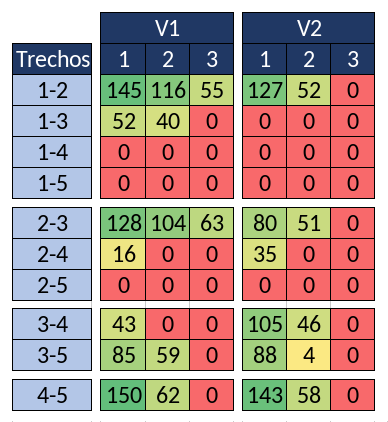
\includegraphics[width=\linewidth]{img/exemplo1.png}
		\caption{Autorizados [Variável $Y$]}
		\label{fig:auto_assig_a}
	\end{subfigure}\hspace{5mm}
	\begin{subfigure}[b]{0.35\linewidth}
		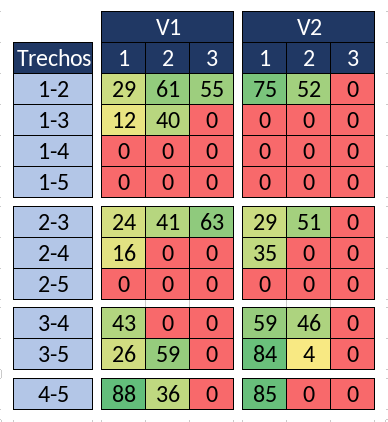
\includegraphics[width=\linewidth]{img/exemplo2.png}
		\caption{Reservados [Variável $X$]}
		\label{fig:auto_assig_b}
	\end{subfigure}
	\caption{Solução factível para os assentos Autorizados e assentos Reservados}
	\label{fig:auto_assig}
\end{figure}

Observe a linha correspondente ao trecho 1-2 do tipo de assento $V_2$ na tabela \ref{fig:auto_assig_b}, veja que a classe reservada mais barata foi a classe 2 com valor de 52, por este motivo na tabela \ref{fig:auto_assig_a} na mesma posição o valor deverá ser igual ou maior que 52, que neste caso é o mesmo valor; Agora observe para o mesmo trecho para o tipo de assento $V_1$ classe 3 em ambas as tabelas acontece a mesma coisa, esse comportamento é garantido pela restrição \ref{eq: m1_autho_mayor_assig_1er_class}. Agora não vamos olhar para a classe mais barata, vamos olhar para qualquer outra, por exemplo, para o mesmo trecho veja a classe 1 do tipo de assento $V_1$ da tabela \ref{fig:auto_assig_b} com valor 29, se quiséssemos saber o valor correspondente na tabela \ref{fig:auto_assig_a} deveríamos adicionar a classe imediata menor (à direita) da classe 1 na tabela \ref{fig:auto_assig_a}, neste caso seria a classe 2 com valor 116, e some o valor da classe 1 da tabela \ref{fig:auto_assig_b}, que já sabemos que é 29, assim, o valor buscado será maior ou igual a $116+29 = 145$, como visto em tabela \ref{fig:auto_assig_a}, lembre-se que nessa posição o valor mínimo será o calculado, mas poderá assumir um valor superior. Esta última situação é controlada pela restrição \ref{eq: m1_autho_mayor_assig_mas_autho}.

% Suponha que você tem um trecho não adjacente E1-E3, e que esse trecho contém outros trechos E1-E2 e E2-E3. Para esta situação, a classe mais barata ativada no trecho E1-E3 deverá ser a classe mais barata ativada nos trechos E1-E2 e E2-E3. Isso é feito com o objetivo de que as combinações dos preços dos bilhetes por trechos não sejam mais econômicos do que o preço de um bilhete direto. Para alcançar isso, é criada uma variável binária para cada trecho não adjacente ($\gamma$), que será ativada, ou tomará o valor de 1, quando as passagem autorizadas $"Y"$ (ou assentos a serem disponibilizados para venda) de uma classe desse trecho, de um tipo de assento e de um período, forem diferentes de zero e tomará o valor de zero caso contrário. Esse comportamento será controlado pela restrição \ref{eq: m1_activ_bin_autho}.

% Uma vez calculados os valores para $\gamma$ dos trechos não adjacentes, a restrição \ref{eq: m1_autho_igualar_trecho_maior} fará com que as classes de controle de todos os trechos contidos em cada trecho não adjacente sejam $0$ ou, no mínimo $1$. Assim, quando a classe de controle do trecho não adjacente assumir um valor de $\gamma = 0$, essa classe será $0$ para os trechos contidos. Por outro lado, se a classe de controle do trecho não adjacente assumir o valor de $\gamma = 1$, então essa classe tomará, no mínimo, o valor de $1$ para todos os trechos contidos.

% Para um melhor entendimento, suponha um trem com 1 tipo de assento que passa por 3 estações, $E_1$, $E_2$ e $E_3$, e tem um horizonte de reserva de um único período. Sob esta situação, o trecho não adjacente seria $"E_1-E_3"$ e os trechos contidos seriam $"E_1-E_2"$ e $"E_2-E_3"$. Agora imagine que cada trecho tem 6 classes diferentes ($c_1, c_2, c_3, c_4, c_5, c_6$), onde o preço  de  $c_1 \geq c_2 \geq c_3 \geq c_4 \geq c_5 \geq c_6$, e que as autorizações para o trecho não adjacente (variável $Y$) tomam os valores mostrados na tabela \ref{fig: exemplo_sip}:


% \begin{small}
% \begin{longtable}[c]{c|cccc|}
% 	\cline{2-5}
% 	\textbf{}                                                                   & \multicolumn{2}{c|}{\cellcolor[HTML]{2E886B}\textbf{$E_1-E_3$}}                                                                                   & \multicolumn{1}{c|}{\cellcolor[HTML]{5CD7E0}$E_1-E_2$}                    & \cellcolor[HTML]{5CD7E0}$E_2-E_3$ \\ \hline
% 	\endfirsthead
% 	\endhead
% 	\rowcolor[HTML]{1D5B73} 
% 	\multicolumn{1}{|c|}{\cellcolor[HTML]{1D5B73}{\color[HTML]{FFFFFF} Classe}} & \multicolumn{1}{c|}{\cellcolor[HTML]{1D5B73}{\color[HTML]{FFFFFF} Y}} & \multicolumn{1}{c|}{\cellcolor[HTML]{1D5B73}{\color[HTML]{FFFFFF} $\gamma$}} & \multicolumn{1}{c|}{\cellcolor[HTML]{1D5B73}{\color[HTML]{FFFFFF} Y}} & {\color[HTML]{FFFFFF} Y}      \\ \hline
% 	\multicolumn{1}{|c|}{\cellcolor[HTML]{1D5B73}{\color[HTML]{FFFFFF} $c_1$}}     & 10                                                                    & {\color[HTML]{00b300} 1}                                              & ${\color[HTML]{00b300} 1} \leq Y \leq Q $                              & ${\color[HTML]{00b300} 1} \leq Y \leq Q $                         \\ \cline{1-1}
% 	\multicolumn{1}{|c|}{\cellcolor[HTML]{1D5B73}{\color[HTML]{FFFFFF} $c_2$}}     & 9                                                                     & {\color[HTML]{00b300} 1}                                              & ${\color[HTML]{00b300} 1} \leq Y \leq Q $                                                                 & ${\color[HTML]{00b300} 1} \leq Y \leq Q $                         \\ \cline{1-1}
% 	\multicolumn{1}{|c|}{\cellcolor[HTML]{1D5B73}{\color[HTML]{FFFFFF} $c_3$}}     & 5                                                                     & {\color[HTML]{00b300} 1}                                              & ${\color[HTML]{00b300} 1} \leq Y \leq Q $                                                                 & ${\color[HTML]{00b300} 1} \leq Y \leq Q $                         \\ \cline{1-1}
% 	\multicolumn{1}{|c|}{\cellcolor[HTML]{1D5B73}{\color[HTML]{FFFFFF} $c_4$}}     & 5                                                                     & {\color[HTML]{00b300} 1}                                              & ${\color[HTML]{00b300} 1} \leq Y \leq Q $                                                                 & ${\color[HTML]{00b300} 1} \leq Y \leq Q $                         \\ \cline{1-1}
% 	\multicolumn{1}{|c|}{\cellcolor[HTML]{1D5B73}{\color[HTML]{FFFFFF} $c_5$}}     & 0                                                                     & {\color[HTML]{FE0000} 0}                                              & ${\color[HTML]{FE0000} 0} \leq Y \leq {\color[HTML]{FE0000} 0} $                                          & ${\color[HTML]{FE0000} 0} \leq Y \leq {\color[HTML]{FE0000} 0} $                        \\ \cline{1-1}
% 	\multicolumn{1}{|c|}{\cellcolor[HTML]{1D5B73}{\color[HTML]{FFFFFF} $c_6$}}     & 0                                                                     & {\color[HTML]{FE0000} 0}                                              & ${\color[HTML]{FE0000} 0} \leq Y \leq {\color[HTML]{FE0000} 0} $                                          & ${\color[HTML]{FE0000} 0} \leq Y \leq {\color[HTML]{FE0000} 0} $                        \\ \hline
% 	\caption{Exemplo simplificado do funcionamento da restrição \ref{eq: m1_autho_igualar_trecho_maior}}
% 	\label{tab: exemplo_sip}
% \end{longtable}
% \end{small}



% Para o trecho $"E_1-E_3"$, note que quando $Y \neq 0$, $\gamma = 1$ e quando $Y = 0$, $\gamma = 0$ (controlado pela restrição \ref{eq: m1_activ_bin_autho}). Agora observe que, quando $ \gamma = 1$ para uma certa classe, os trechos $E_1-E_2$ e $E_2-E_3$ assumem valores entre 1 e um número suficientemente grande ($1 \le Y \leq Q$) neste caso a capacidade do trem, o que indica que os assentos a serem disponibilizados para essa classe nesses trechos não podem ser zero. Por outro lado, quando $\gamma = 0$, os trechos menores devem zerar a classe correspondente com ($0 \leq Y \leq 0$), ou seja, não se deve disponibilizar assentos com essa classe (controlado pela restrição \ref{eq: m1_autho_igualar_trecho_maior}). Deve-se esclarecer que as classe de controle dos trechos contidos, apenas imitam o comportamento da classe não adjacente correspondente, e não os valores que esta assume.

A restrição \ref{eq: m1_assig_menor_dem} garante que a quantidade de passagens reservadas não ultrapasse a demanda para cada trecho de cada classe de cada tipo de assento e em cada período no horizonte de reserva.

A restrição  \ref{eq: m1_activ_bin_autho} é utilizada para determinar quando a variável de decisão $Y$ assume valores diferentes de zero e quando não. Assim, $\gamma $ toma o valor de 1 no primeiro caso e 0 no segundo.

Uma condição importante estabelece que uma classe pode ser reservada desde que essa mesma classe já tenha sido reservada em períodos anteriores. Para isso, definem-se as restrições \ref{eq: m1_binaria_alpha} e \ref{eq: m1_assig_last_periodo}, onde a primeira busca atribuir o valor 1 à variável $\alpha_{ijvkt}$ quando $X_{ijvkt}$ assume um valor diferente de zero, e atribuir 0 caso contrário; essa restrição possui a mesma estrutura e raciocínio da restrição \ref{eq: m1_activ_bin_autho}.

Agora, a restrição \ref{eq: m1_assig_last_periodo} garante que uma certa variável binária $\alpha_{ijvkt}$ tomará o valor 1 se, e somente se, no período anterior ( $\alpha_{i,j,v,k,t+1}$) também assumiu o valor 1; caso contrário, ela fica livre para tomar qualquer valor, 0 ou 1. Isso significa que só é possível reservar uma certa classe se essa mesma classe foi reservada no período anterior. Vejamos um exemplo:


\begin{figure}[h!]
    \centering
    \begin{subfigure}[b]{0.40\linewidth}
		\begin{tikzpicture}
            \node[anchor=south west, inner sep=0] (image1) at (-0.33,0.5) {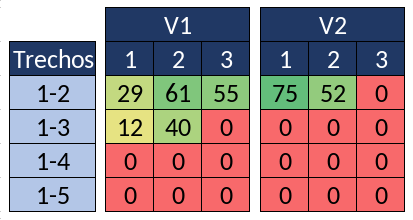
\includegraphics[width=\linewidth]{img/assig_t1.png}};
			\draw[purple, line width=0.7mm, rounded corners=5pt] (3.7,2.23) rectangle (5.46,2.83);
        \end{tikzpicture}
        \caption{Assentos Reservados $[X]$, em $t = 1$}
        \label{fig:assig_t1}
    \end{subfigure}\hspace{5mm}
    \begin{subfigure}[b]{0.40\linewidth}
        \begin{tikzpicture}
            \node[anchor=south west, inner sep=0] (image1) at (-0.33,0.5) {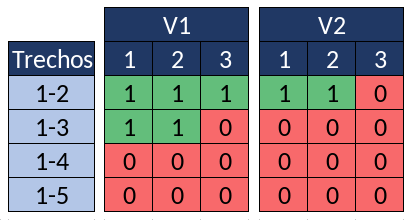
\includegraphics[width=\linewidth]{img/bx_t1.png}};
            \draw[blue, line width=0.8mm] (2.5,2) circle (0.35cm); % Ajusta las coordenadas y radio
			\draw[purple, line width=0.7mm, rounded corners=5pt] (3.7,2.23) rectangle (5.46,2.83);
        \end{tikzpicture}
        \caption{$\alpha$, em $t = 1$}
        \label{fig:alpha_t1}
    \end{subfigure}
    \begin{subfigure}[b]{0.40\linewidth}
		\begin{tikzpicture}
			\node[anchor=south west, inner sep=0] (image3) at (0.16,0.03) {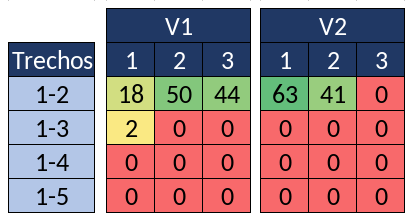
\includegraphics[width=\linewidth]{img/assig_t0.png}};
			\draw[blue, line width=0.7mm] (3,1.5) circle (0.35cm); % Ajusta las coordenadas y radio
        \end{tikzpicture}
		\caption{Assentos Reservados $[X]$, em $t = 0$}
        \label{fig:assig_t0}
    \end{subfigure}\hspace{5mm}
    \begin{subfigure}[b]{0.40\linewidth}
        \begin{tikzpicture}
            \node[anchor=south west, inner sep=0] (image2) at (0.16,0.03) {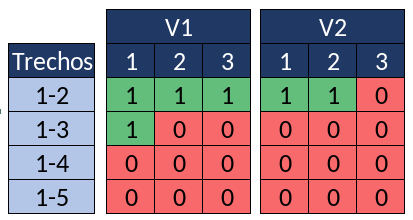
\includegraphics[width=\linewidth]{img/bx_to.png}};
            \draw[blue, line width=0.7mm] (3,1.5) circle (0.35cm); % Ajusta las coordenadas y radio
        \end{tikzpicture}
        \caption{$\alpha$, em $t = 0$}
        \label{fig:alpha_t0}
    \end{subfigure}
    \caption{Exemplo: Restrições Fulfillments over periods}
    \label{fig:restricao_fulfillments}
\end{figure}


Lembre que $t=0$ é a data de partida do trem, ou seja, quanto maior for o valor de $t$, mais longe estará da data de partida. Assim, $t=1$ será o período exatamente anterior a $t=0$.

Para cada trecho, tipo de assento e classe dados na figura \ref{fig:restricao_fulfillments}, suponha que: a figura \ref{fig:assig_t1} é uma solução factível que representa a quantidade de assentos reservados para o período $t=1$; a figura \ref{fig:alpha_t1}  é a variável binária $\alpha_{ijvkt}$, que mostra 1 sempre que a quantidade de assentos reservados for diferente de zero em $t=1$ e mostra zero caso contrário (controlado pela restrição \ref{eq: m1_binaria_alpha}). As figuras \ref{fig:assig_t0} e \ref{fig:alpha_t0} representam o mesmo que as figuras \ref{fig:assig_t1} e \ref{fig:alpha_t1}, mas para o período $t=0$.

Observe que as posições na figura \ref{fig:alpha_t0} tomarão o valor zero sempre que, na figura \ref{fig:alpha_t1}, essa posição também for zero. Isso significa que, se a classe do período anterior for zero, então a do período atual também será zero. Note também que, quando o valor na figura \ref{fig:alpha_t1} é 1, na figura \ref{fig:alpha_t0} o valor poderá ser 0 ou 1. Por exemplo, para o trecho $1-3$ do tipo de assento $v_1$ e classe 2, note que na figura \ref{fig:alpha_t1} o valor é 1 e na figura \ref{fig:alpha_t0} é zero, o que significa que a classe 2 foi reservada no período anterior, mas no período atual não foi.


Outra condição especial deste problema está relacionada à disponibilização dos preços dos bilhetes ao longo do tempo. Esses preços devem seguir uma lógica contínua, sem oscilações. Em outras palavras, os preços dos bilhetes devem sempre aumentar conforme a data de partida do trem se aproxima. A restrição \ref{eq: m1_fulfill_periodo} é responsável por garantir que essa condição seja atendida.

Por outro lado, a restrição \ref{eq: m1_binaria_Beta} e \ref{eq: m1_binaria_Beta_last} cumprem a mesma função de encontrar a última classe que foi disponibilizada para venda em um determinado trecho, período e tipo de assento. No entanto, a restrição \ref{eq: m1_binaria_Beta_last} é aplicada sempre que se analisa a classe mais barata, e, em outros casos, usa-se a restrição \ref{eq: m1_binaria_Beta}. Assim, essas duas equações atribuem o valor 1 à variável $\beta_{ijvkt}$ sempre que a classe atual $k$ seja a classe mais barata disponibilizada para venda no trecho $(i,j)$, tipo de assento $v$, e período $t$; caso contrário, atribui-se o valor zero. Essa restrição é necessária para aplicar as restrições \ref{eq: m1_preco_estacao_inicio} e \ref{eq: m1_preco_combinacao_rotas_contidas}.

Vamos usar o mesmo exemplo da figura \ref{fig: exemplo_sip}, considerando apenas o trecho $E_1-E_3$ e adicionando a variável binária $\beta$.

\begin{figure}[h!]
	\centering
	\begin{subfigure}[b]{0.35\linewidth}
		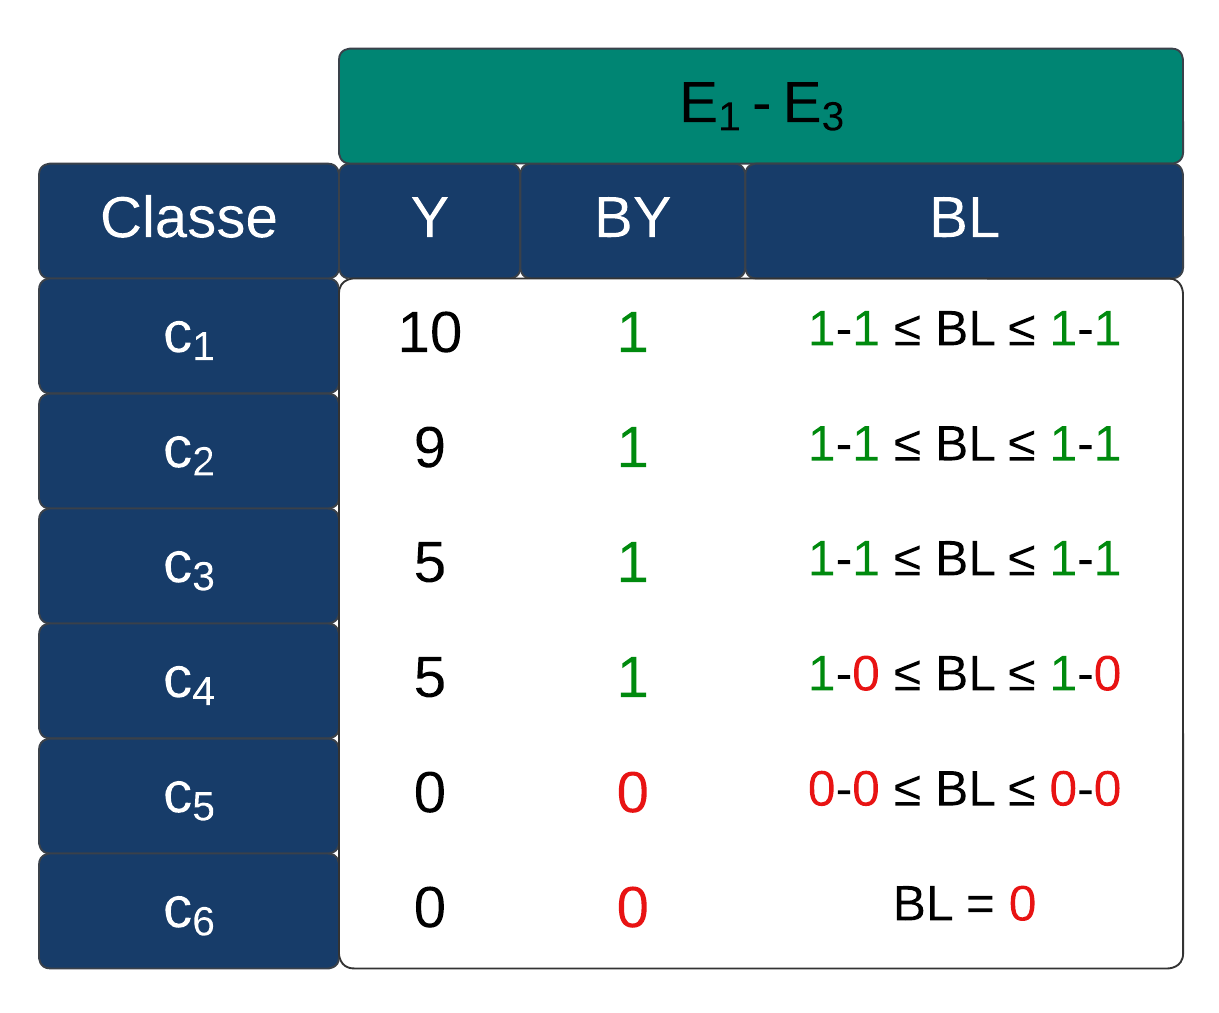
\includegraphics[width=\linewidth]{img/BL_1.png}
		\caption{Cálculo Variável $\beta$}
		\label{fig:Beta_1}
	\end{subfigure}\hspace{5mm}
	\begin{subfigure}[b]{0.35\linewidth}
		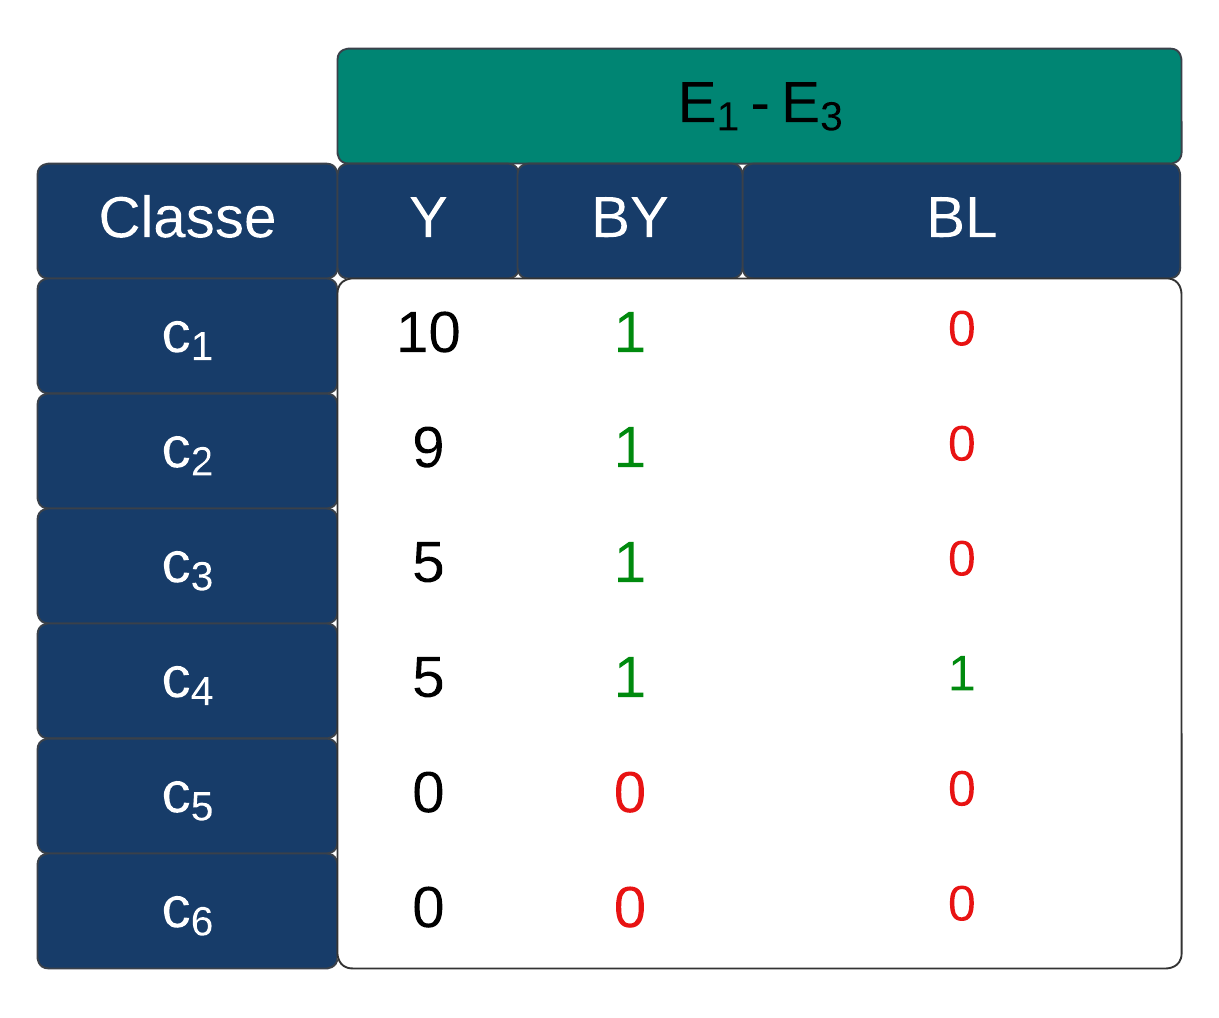
\includegraphics[width=\linewidth]{img/BL_2.png}
		\caption{Resultado Variável $\beta$}
		\label{fig:Beta_2}
	\end{subfigure}
	\caption{Exemplo para as restrições \ref{eq: m1_binaria_Beta} e \ref{eq: m1_binaria_Beta_last}}
	\label{fig:Beta}
\end{figure}

Na figura \ref{fig:Beta_1}, vemos que, para a classe mais barata $c_6$, $\beta=\gamma=0$. Agora, para o restante das classes, realiza-se um cálculo com base nos valores de $\gamma$. Por exemplo, para a classe $c_1$, o cálculo seria: $\gamma$ de $c_1$ menos $\gamma$ da próxima classe, ou seja, $\gamma$ de $c_2$, o que resulta em $1-1$. Note, além disso, que para a classe $c_4$, fazendo o mesmo cálculo, o resultado é 1, como mostrado na figura \ref{fig:Beta_2}, e observe que essa classe é a última que possui um valor diferente de zero em $\gamma$.


\begin{figure}[!ht]
	\begin{center}
		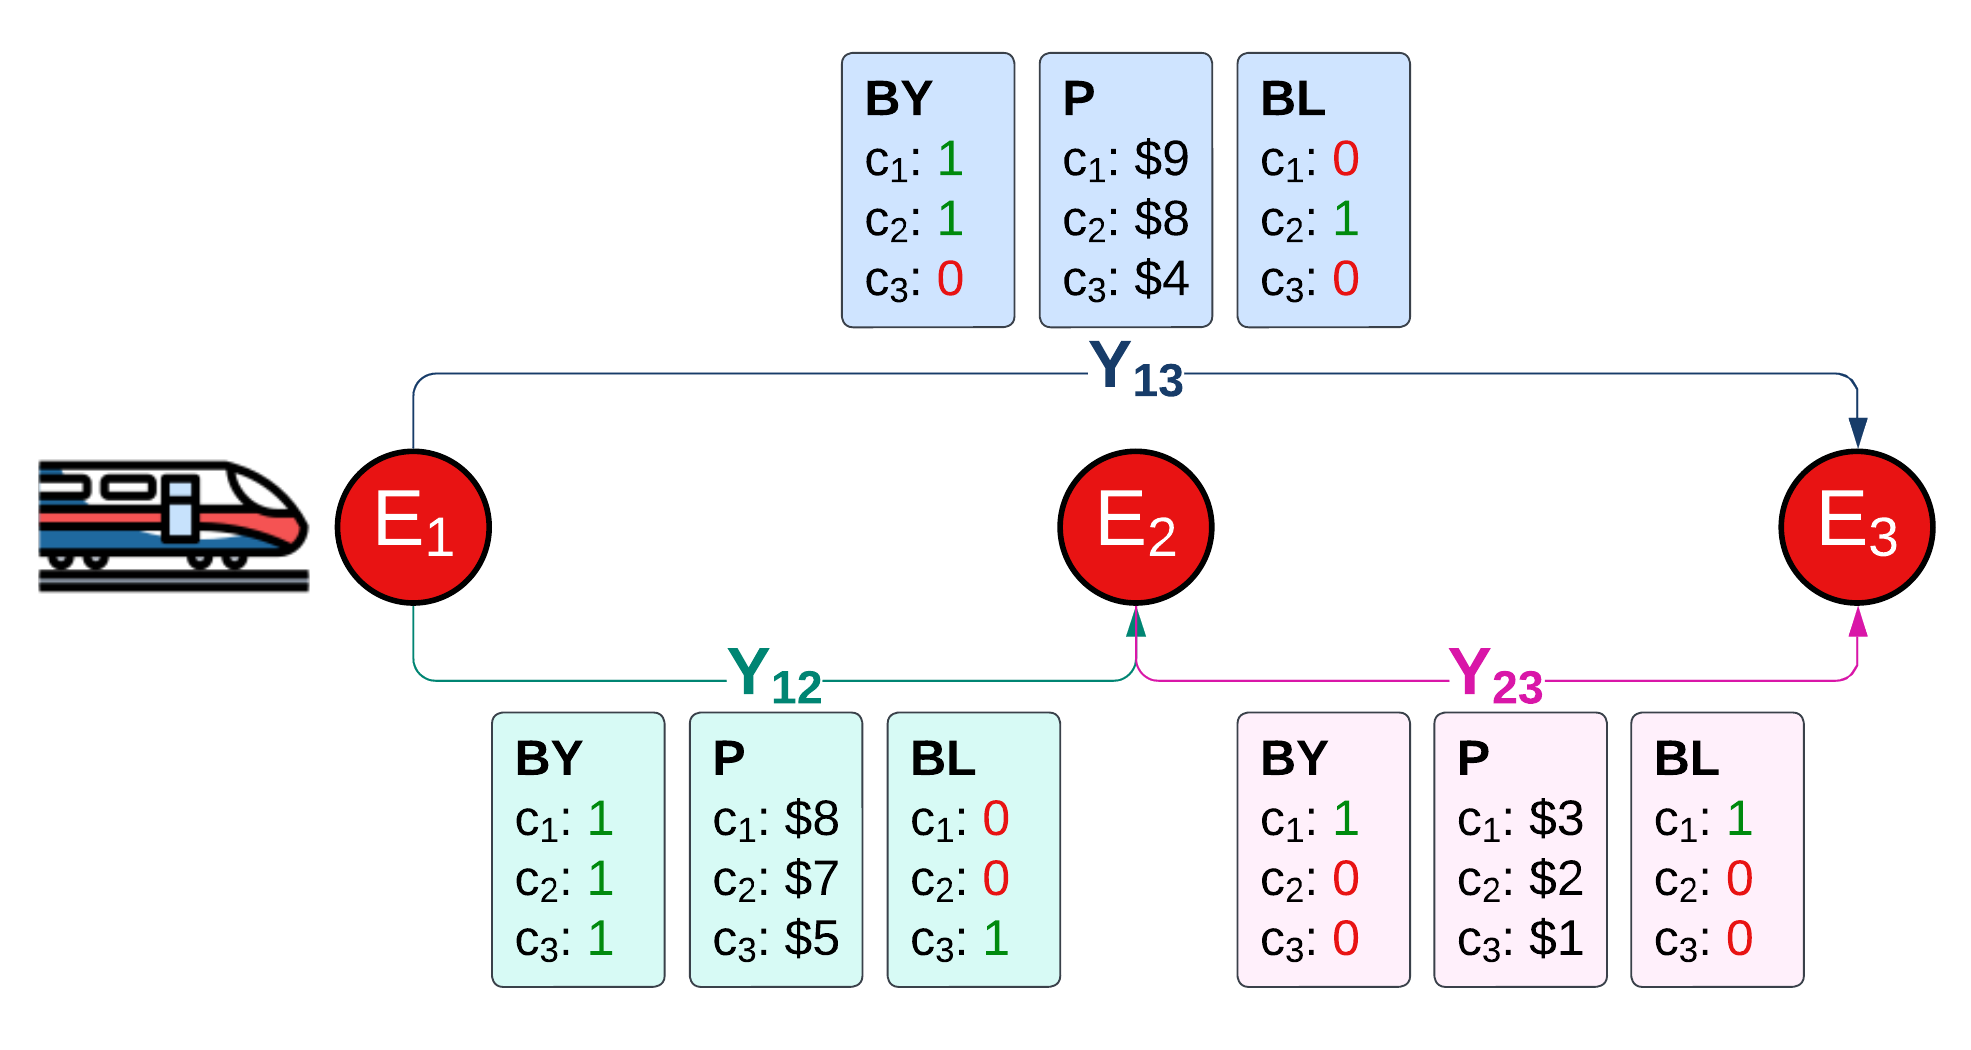
\includegraphics[scale=0.2]{img/fulfill.png}
		\caption{Exemplo para as restrições \ref{eq: m1_preco_estacao_inicio} e \ref{eq: m1_preco_combinacao_rotas_contidas}}
		% Fonte:~\cite{khaksar2013genetic}}
		\label{fig: fulfill}
	\end{center}
\end{figure}

Dentro do problema, é necessário garantir que, para todos os trechos com a mesma estação de origem, os trechos mais curtos disponibilizados para venda sejam mais baratos que os trechos mais longos. Isso é para evitar que passageiros comprem bilhetes para um trecho maior e desembarquem em estações anteriores. Por exemplo, se uma pessoa quer ir da estação $E_1$ para a estação $E_2$, mas percebe que o preço para ir de $E_1$ a $E_3$ é mais barato, então essa pessoa comprará o bilhete de $E_1$ a $E_3$ e desembarcará na estação $E_2$. Essa situação é controlada pela restrição \ref{eq: m1_preco_estacao_inicio}. 

Vamos ver um exemplo mais claro: na figura \ref{fig: fulfill}, temos três estações, assumindo um único período e um único tipo de assento, além de três classes para cada trecho ($c_1, c_2, c_3$). Note que $\gamma$ e $\beta$ são as variáveis binárias explicadas anteriormente, e $P$ representa o preço de cada classe de controle. Para este caso, a restrição \ref{eq: m1_preco_estacao_inicio} pode ser aplicada aos trechos $(E_1-E_2)$ e $(E_1-E_3)$.

Observe como o produto da soma do preço $P$ e da variável $\beta$ ativa o preço da classe mais barata ($c_3$ com valor de \$7) em $(E_1-E_2)$, e o produto da soma de $(E_1-E_3)$ ativa o preço da classe $c_2$ (com valor de \$8). No final, teríamos que \$7 deve ser menor ou igual a \$8, o que está garantindo que o trecho $(E_1-E_2)$ seja mais barato que o trecho $(E_1-E_3)$.

Note a importância do valor da variável $\beta$, que é responsável por "habilitar apenas os preços" das classes mais baratas disponibilizadas para a venda.

Além do mencionado anteriormente, também deve-se garantir que todas as possíveis combinações dos preços mais baratos dos trechos contidos dentro dos trechos não adjacentes sejam maiores ou iguais ao preço desse trecho não adjacente. Essa situação é controlada pela restrição \ref{eq: m1_preco_combinacao_rotas_contidas}.

Para dar um exemplo, analisemos novamente a figura \ref{fig: fulfill} e identifiquemos os trechos não adjacentes e os trechos que estes contêm. Note que o trecho $(E_1-E_3)$ seria o único trecho não adjacente e contém os trechos $(E_1-E_2)$ e $(E_2-E_3)$. Portanto, precisamos garantir que a soma das classes mais baratas disponibilizadas em $(E_1-E_2)$ e $(E_2-E_3)$ seja maior ou igual à classe mais barata disponibilizada em $(E_1-E_3)$. Em termos numéricos, teríamos que $5+3 \geq 8$. Assim, este exemplo satisfaz nossa restrição.

As restrições de \ref{eq: m1_ini_assig} e \ref{eq: m1_ini_disponi} são usadas para inicializar a restrição \ref{eq: m1_disponi} quando \(i = 1\). E as restrições de \ref{eq: m1_dom_assig} a \ref{eq: m1_dom_bin_nadja} representam o domínio das variáveis.


\section{Segunda modelagem: Demanda Comportamental} \label{sec: modelagemComportamental}

Até agora, falamos de uma demanda independente para o modelo, mas agora trabalharemos com uma demanda comportamental. A demanda comportamental está mais próxima da realidade do que a demanda independente. Veja o seguinte exemplo:

Suponhamos para este caso que temos um trecho $(1-2)$ e três classes $(c_1, c_2, c_3)$, onde o preço de $c_1 > c_2 > c_3$, além, cada classe terá uma demanda de 10, 20 e 30, respectivamente.

\begin{figure}[h!]
	\centering
	\begin{subfigure}[b]{0.40\linewidth}
		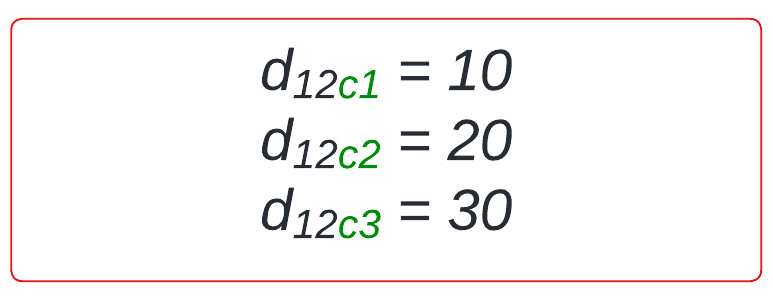
\includegraphics[width=\linewidth]{img/dem_indepen.png}
		\caption{Demanda Independente [$d$]}
		\label{fig:dem_indepen}
	\end{subfigure}\hspace{5mm}
	\begin{subfigure}[b]{0.40\linewidth}
		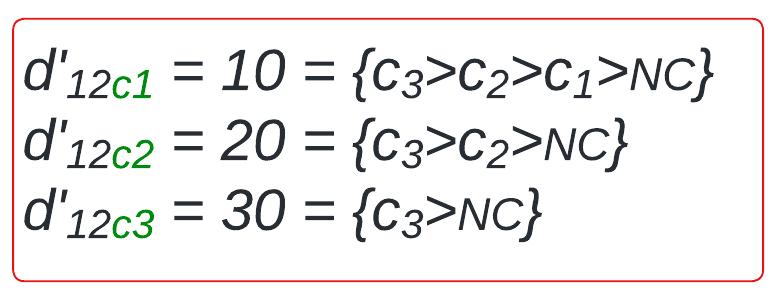
\includegraphics[width=\linewidth]{img/dem_compo.png}
		\caption{Demanda Comportamental [$d'$]}
		\label{fig:dem_comporta}
	\end{subfigure}
	\caption{Exemplo: Tipos de Demanda}
	\label{fig: tipos_demanda}
\end{figure}


Para interpretar a demanda independente, podemos dizer (segundo a figura \ref{fig:dem_indepen}) que: existem 10 pessoas dispostas a comprar passagens \textbf{a um preço} de $c_1$, 20 pessoas a comprar \textbf{a um preço} de $c_2$ e 30 pessoas a comprar \textbf{a um preço} de $c_3$. No entanto, se as 10 pessoas dispostas a pagar $c_1$ encontrarem um melhor valor no momento da compra (por exemplo, $c_3$), essas pessoas prefeririam não comprar, mesmo quando encontram um preço mais barato. Situação que, na realidade, não faria sentido.

Por outro lado, temos a demanda comportamental, denotada como $d'$, que esta representada com uma lista de preferência, conforme visto na figura \ref{fig:dem_comporta}. Esta lista significa que, por exemplo, 10 pessoas estão dispostas a comprar \textbf{até um preço} com valor $c_1$, 20 pessoas estão dispostas a comprar \textbf{até um preço} de $c_2$ e 30 pessoas estão dispostas a comprar \textbf{até um preço} de $c_3$.

O funcionamento seria o seguinte: imagine que as 10 pessoas dispostas a comprar até um valor de $c_1$ vão tentar comprar primeiro a um valor mais barato, neste caso $c_3$. Se $c_3$ não estiver disponível, elas procurariam assentos com valor $c_2$. Se $c_2$ também não estiver disponível, subiriam na lista e procurariam passagens com valor de $c_1$. Se estes não estiverem disponíveis, então não comprariam. Note que esse comportamento é o que comumente se usa na realidade.

Agora vejamos como o modelo leria esse novo comportamento. Para isso, calculemos a nova demanda potencial: 

para $c_1$, vejamos a lista e notemos quem está disposto a pagar por esse valor.
\begin{figure}[!ht]
	\begin{center}
		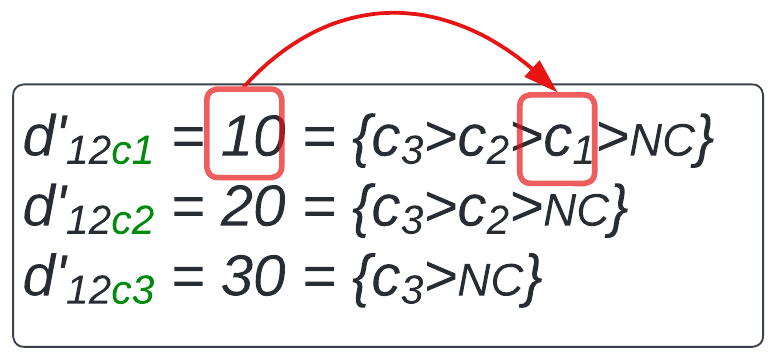
\includegraphics[scale=0.24]{img/dem_compo_c1.png}
		\caption{Exemplo: Demanda comportamental para a classe $c_1$}
		% Fonte:~\cite{khaksar2013genetic}}
		\label{fig: exemplo_dem_c1}
	\end{center}
\end{figure}

Segundo a figura \ref{fig: exemplo_dem_c1}, apenas 10 possíveis passageiros estão dispostos a pagar esse valor.

Agora vamos ver quem está disposto a pagar um valor por um bilhete da classe $c_2$:
\begin{figure}[!ht]
	\begin{center}
		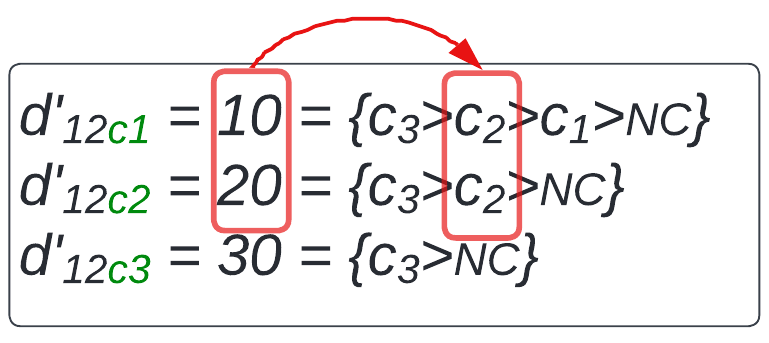
\includegraphics[scale=0.24]{img/dem_compo_c2.png}
		\caption{Exemplo: Demanda comportamental para a classe $c_2$}
		% Fonte:~\cite{khaksar2013genetic}}
		\label{fig: exemplo_dem_c2}
	\end{center}
\end{figure}

Neste caso, 30 possíveis pessoas estariam dispostas a pagar esse valor. Observe que, de esta nova demanda, 10 pessoas correspondentes à demanda de $c_1$ também estariam dispostas a comprar pelo valor da classe $c_2$.

Por último, para a classe mais barata c3, veja a figura \ref{fig: exemplo_dem_c3}.
\begin{figure}[!ht]
	\begin{center}
		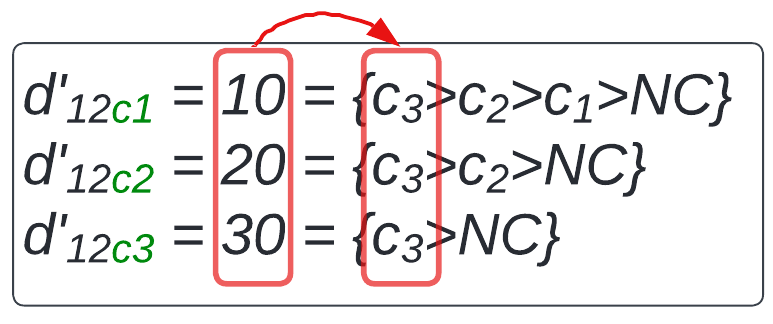
\includegraphics[scale=0.24]{img/dem_compo_c3.png}
		\caption{Exemplo: Demanda comportamental para a classe $c_3$}
		% Fonte:~\cite{khaksar2013genetic}}
		\label{fig: exemplo_dem_c3}
	\end{center}
\end{figure}
Note que, neste caso, 60 pessoas estariam dispostas a pagar um bilhete da classe $c_3$, ou seja, toda a demanda da rota $(1-2)$ compraria pelo valor mais barato se este estivesse disponível.

Assim, a demanda potencial comportamental para o modelo seria como se apresenta na figura \ref{fig: exemplo_dem_poten}.
\begin{figure}[!ht]
	\begin{center}
		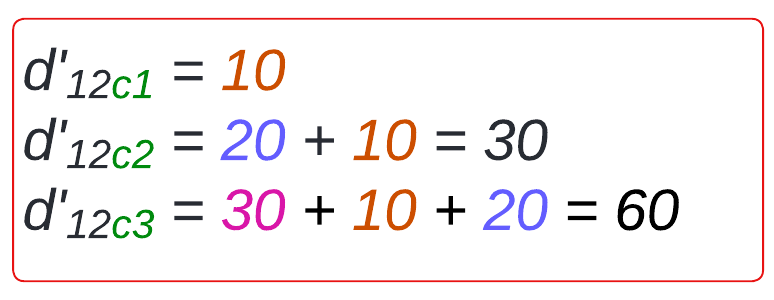
\includegraphics[scale=0.24]{img/dem_compo_poten.png}
		\caption{Exemplo: Demanda comportamental total Potencial}
		% Fonte:~\cite{khaksar2013genetic}}
		\label{fig: exemplo_dem_poten}
	\end{center}
\end{figure}
No entanto, é importante lembrar que a demanda potencial inicial era de 60 pessoas, mas até este ponto, a demanda poderia ser maior, pois a demanda de cada classe comercial agora é o acúmulo das demandas das classes mais caras. Essa situação precisa ser controlada para não criar uma demanda inexistente; para isso, serão consideradas as seguintes restrições, relacionando neste caso as variáveis de decisão de assentos reservados:

\begin{align}
    & X_{12\textcolor[rgb]{0.0588, 0.5412, 0.4275}{c_1}} \leq d'_{12\textcolor[rgb]{0.0588, 0.5412, 0.4275}{c_1}} = 10                        \label{eq: dem_asiig_c1} \\
    & X_{12\textcolor[rgb]{0.0588, 0.5412, 0.4275}{c_2}} \leq d'_{12\textcolor[rgb]{0.0588, 0.5412, 0.4275}{c_2}} = 30                        \label{eq: dem_asiig_c2} \\
    & X_{12\textcolor[rgb]{0.0588, 0.5412, 0.4275}{c_3}} \leq d'_{12\textcolor[rgb]{0.0588, 0.5412, 0.4275}{c_3}} = 60                      \label{eq: dem_asiig_c3} \\
    & X_{12\textcolor[rgb]{0.0588, 0.5412, 0.4275}{c_1}} + X_{12\textcolor[rgb]{0.0588, 0.5412, 0.4275}{c_2}} \leq d'_{12\textcolor[rgb]{0.0588, 0.5412, 0.4275}{c_2}}  = 30           \label{eq: dem_compo_c2} \\
    & X_{12\textcolor[rgb]{0.0588, 0.5412, 0.4275}{c_1}} + X_{12\textcolor[rgb]{0.0588, 0.5412, 0.4275}{c_2}} + X_{12\textcolor[rgb]{0.0588, 0.5412, 0.4275}{c_3}} \leq d'_{12\textcolor[rgb]{0.0588, 0.5412, 0.4275}{c_3}} = 60 \label{eq: dem_compo_c3}                    
\end{align}

Observe que as restrições de \ref{eq: dem_asiig_c1} até \ref{eq: dem_asiig_c3} são restrições conhecidas que limitam os valores que as passagens reservadas podem assumir, enquanto as restrições \ref{eq: dem_compo_c2} e \ref{eq: dem_compo_c3} são as que nos ajudarão a controlar para não ultrapassarmos a demanda potencial total inicial. 

Por exemplo, se $X_{12\textcolor[rgb]{0.0588, 0.5412, 0.4275}{c_2}}$ assume o valor de 30 (restrição \ref{eq: dem_asiig_c2}), a restrição \ref{eq: dem_compo_c2} garante que $X_{12\textcolor[rgb]{0.0588, 0.5412, 0.4275}{c_1}}$ seja igual a 0, pois a demanda de 10 pessoas correspondente preferiu comprar ao preço da classe $c_2$. A mesma situação ocorreria se $X_{12\textcolor[rgb]{0.0588, 0.5412, 0.4275}{c_3}}$ assumisse o valor de 60 (restrição \ref{eq: dem_asiig_c3}), então a restrição \ref{eq: dem_compo_c3} garantiria que a demanda por $X_{12\textcolor[rgb]{0.0588, 0.5412, 0.4275}{c_1}}$ e $X_{12\textcolor[rgb]{0.0588, 0.5412, 0.4275}{c_2}}$ fosse igual a zero, já que esses clientes decidiram comprar pelo valor da classe $c_3$. Dessa forma, esse conjunto de restrições funcionaria para cada combinação possível das variáveis descritas.

Agora, para formular o modelo completo utilizando a demanda comportamental baseada em faixas de preferência, basta modificar apenas as restrições que controlam a demanda no modelo independente e adicionar as restrições generalizadas descritas no modelo comportamental.

\allowdisplaybreaks
\begin{align}
	& \textcolor{red}{X_{ijvkt} \leq d'_{ijvkt},  \quad \forall (i,j) \in OD / i < j  ,v \in V, k \in K_v, t\in T }                                                                                                 \label{eq: m2_assig_menor_dem}                                                 \\
	& \sum_{k' \in K_v / k' \leq k}X_{i,j,v,k',t} \leq d'_{ijvkt} \quad \forall (i,j) \in OD, v \in V, k \in K_v / k > 1, t\in T                                                                                    \label{eq: m2_dem_compor_acumulacao_class}                                     
\end{align}

As restrições \ref{eq: m2_assig_menor_dem} e \ref{eq: m2_dem_compor_acumulacao_class} representam a generalização das restrições de \ref{eq: dem_asiig_c1} a \ref{eq: dem_compo_c3}. Apenas adicionando essas duas últimas restrições e eliminando a restrição \ref{eq: m1_assig_menor_dem} do modelo independente, obteríamos, em teoria, um modelo com demanda comportamental. No entanto, essa afirmação não é completamente verdadeira. Embora as novas restrições limitem a demanda do modelo de forma que possam ser utilizadas as listas de preferência, o modelo ainda se comportará como um modelo independente.

Isso ocorre porque a demanda independente é um caso particular de todas as combinações possíveis que podem ser geradas ao usar as listas de preferência. Além disso, a demanda independente é o caso que produziria o maior lucro. Lembre-se de que as listas de preferência permitem a flexibilidade de um cliente disposto a pagar mais caro poder adquirir um produto mais barato, caso exista essa possibilidade — algo que a demanda independente não permite. Por isso, já sabemos de antemão que a solução obtida com a demanda comportamental será inferior à solução oferecida pelo modelo independente.

Além disso, é importante destacar que o modelo apresenta um comportamento otimista, pois assume que os clientes dispostos a pagar mais caro sempre chegarão antes daqueles que estão dispostos a pagar menos (devido à formulação da função objetivo).

Portanto, não basta apenas adicionar as restrições \ref{eq: m2_assig_menor_dem} e \ref{eq: m2_dem_compor_acumulacao_class} para afirmar que temos um modelo com demanda comportamental. É necessário, de alguma forma, informar ao modelo que ele deve considerar outras possibilidades "mais realistas" durante a resolução do problema. É nesse ponto que introduzimos as seguintes restrições, que ajudarão a mitigar essa situação:

\allowdisplaybreaks
\begin{align}
	& X_{ijvkt} \leq \left( d'_{ijvkt} \right) \left(\frac{d_{ijvkt}}{d'_{i,j,v,k',t}}\right),  \quad \forall (i,j) \in OD, v \in V, k \in K_v/ k < k', k' < max\{K_v\}, t\in T                                     \label{eq: m2_dem_compor_porcentaje_dem}                                       \\
	\begin{split}
		& X_{i,j,v,k',t} \leq d_{i,j,v,k',t} + \left( d'_{i,j,v,k',t} - \sum_{k \in K_v }\frac{d'_{ijvkt} d_{ijvkt}}{d'_{i,j,v,k',t}} \right),  \quad \forall (i,j) \in OD                                                                                                                         \\
		& v \in V, k' = max\{K_v\}, t\in T                                                                                                                                                                                                                                                         \\
	\end{split}                                                                                                                                                                                                      \label{eq: m2_dem_compor_porcentaje_dem_last}                                                                              
\end{align}


Para essas novas restrições, além da demanda comportamental, também utilizaremos a demanda independente. Assim, na restrição \ref{eq: m2_dem_compor_porcentaje_dem}, o que fazemos é calcular as proporções da demanda independente para as classes de cada trecho, tipo de assento e período. Em seguida, essas proporções são multiplicadas pela demanda comportamental. Esse processo faz com que as demandas comportamentais potenciais para cada classe sejam reduzidas de acordo com as proporções da demanda independente. Dessa forma, garantimos que a solução obtida não seja idêntica à oferecida pelo modelo independente.

Observe que, ao calcular essas proporções, a demanda comportamental é reduzida, o que resulta em uma "perda de demanda". Esse complemento é então somado à classe mais barata do trecho, tipo de assento e período analisado, conforme ilustrado pela restrição \ref{eq: m2_dem_compor_porcentaje_dem_last}. Dessa forma, incentivamos o modelo a utilizar as classes mais baratas. Vamos analisar um exemplo: assuma que há um trecho com três classes para um tipo de assento e um período, e que essas classes possuem parâmetros de demanda independente $d$, conforme mostrado na Tabela \ref{tab: exemplo_ajuste_demanda}.

\begin{table}[h!]
    \centering
    \begin{tabular}{lccccc}
        \toprule
        & Classes & $d$ & \% & $d'$ & \textbf{\% * $d'$} \\
        \midrule
              & $c_1$ & 36 & 34,62\% & 36 & \textbf{12,46} \\
              & $c_2$ & 58 & 55,77\% & 94 & \textbf{52,42} \\
              & $c_3$ & 10 & 9,62\% & 104 & \textbf{10 + 29,12} \\
        \midrule
              & Total & 104 & & & \\
        \bottomrule
    \end{tabular}
    \caption{Exemplo ajuste da demanda comportamental com proporções}
	\label{tab: exemplo_ajuste_demanda}
\end{table}

Observe que a coluna "\%" \, apresenta as proporções calculadas com base na demanda independente $d$. A coluna $d'$ mostra a demanda comportamental potencial, enquanto a coluna "\%*$d'$" \, exibe o produto entre as proporções "\%" \, e a demanda comportamental ($d'$).

Adicionalmente, note que, para a classe mais barata $c_3$, o valor da última coluna é 10 (resultado do produto mencionado) somado a $29.12$. Este último valor representa o complemento da demanda, ou seja, $104-(12,46+52,42+10)$. Esse complemento é redistribuído para a classe mais acessível, garantindo que as regras do modelo sejam atendidas de forma a refletir a alocação proporcional e a flexibilidade comportamental.

\begin{figure}[H]
	\centering
	\begin{subfigure}[b]{0.45\linewidth}
		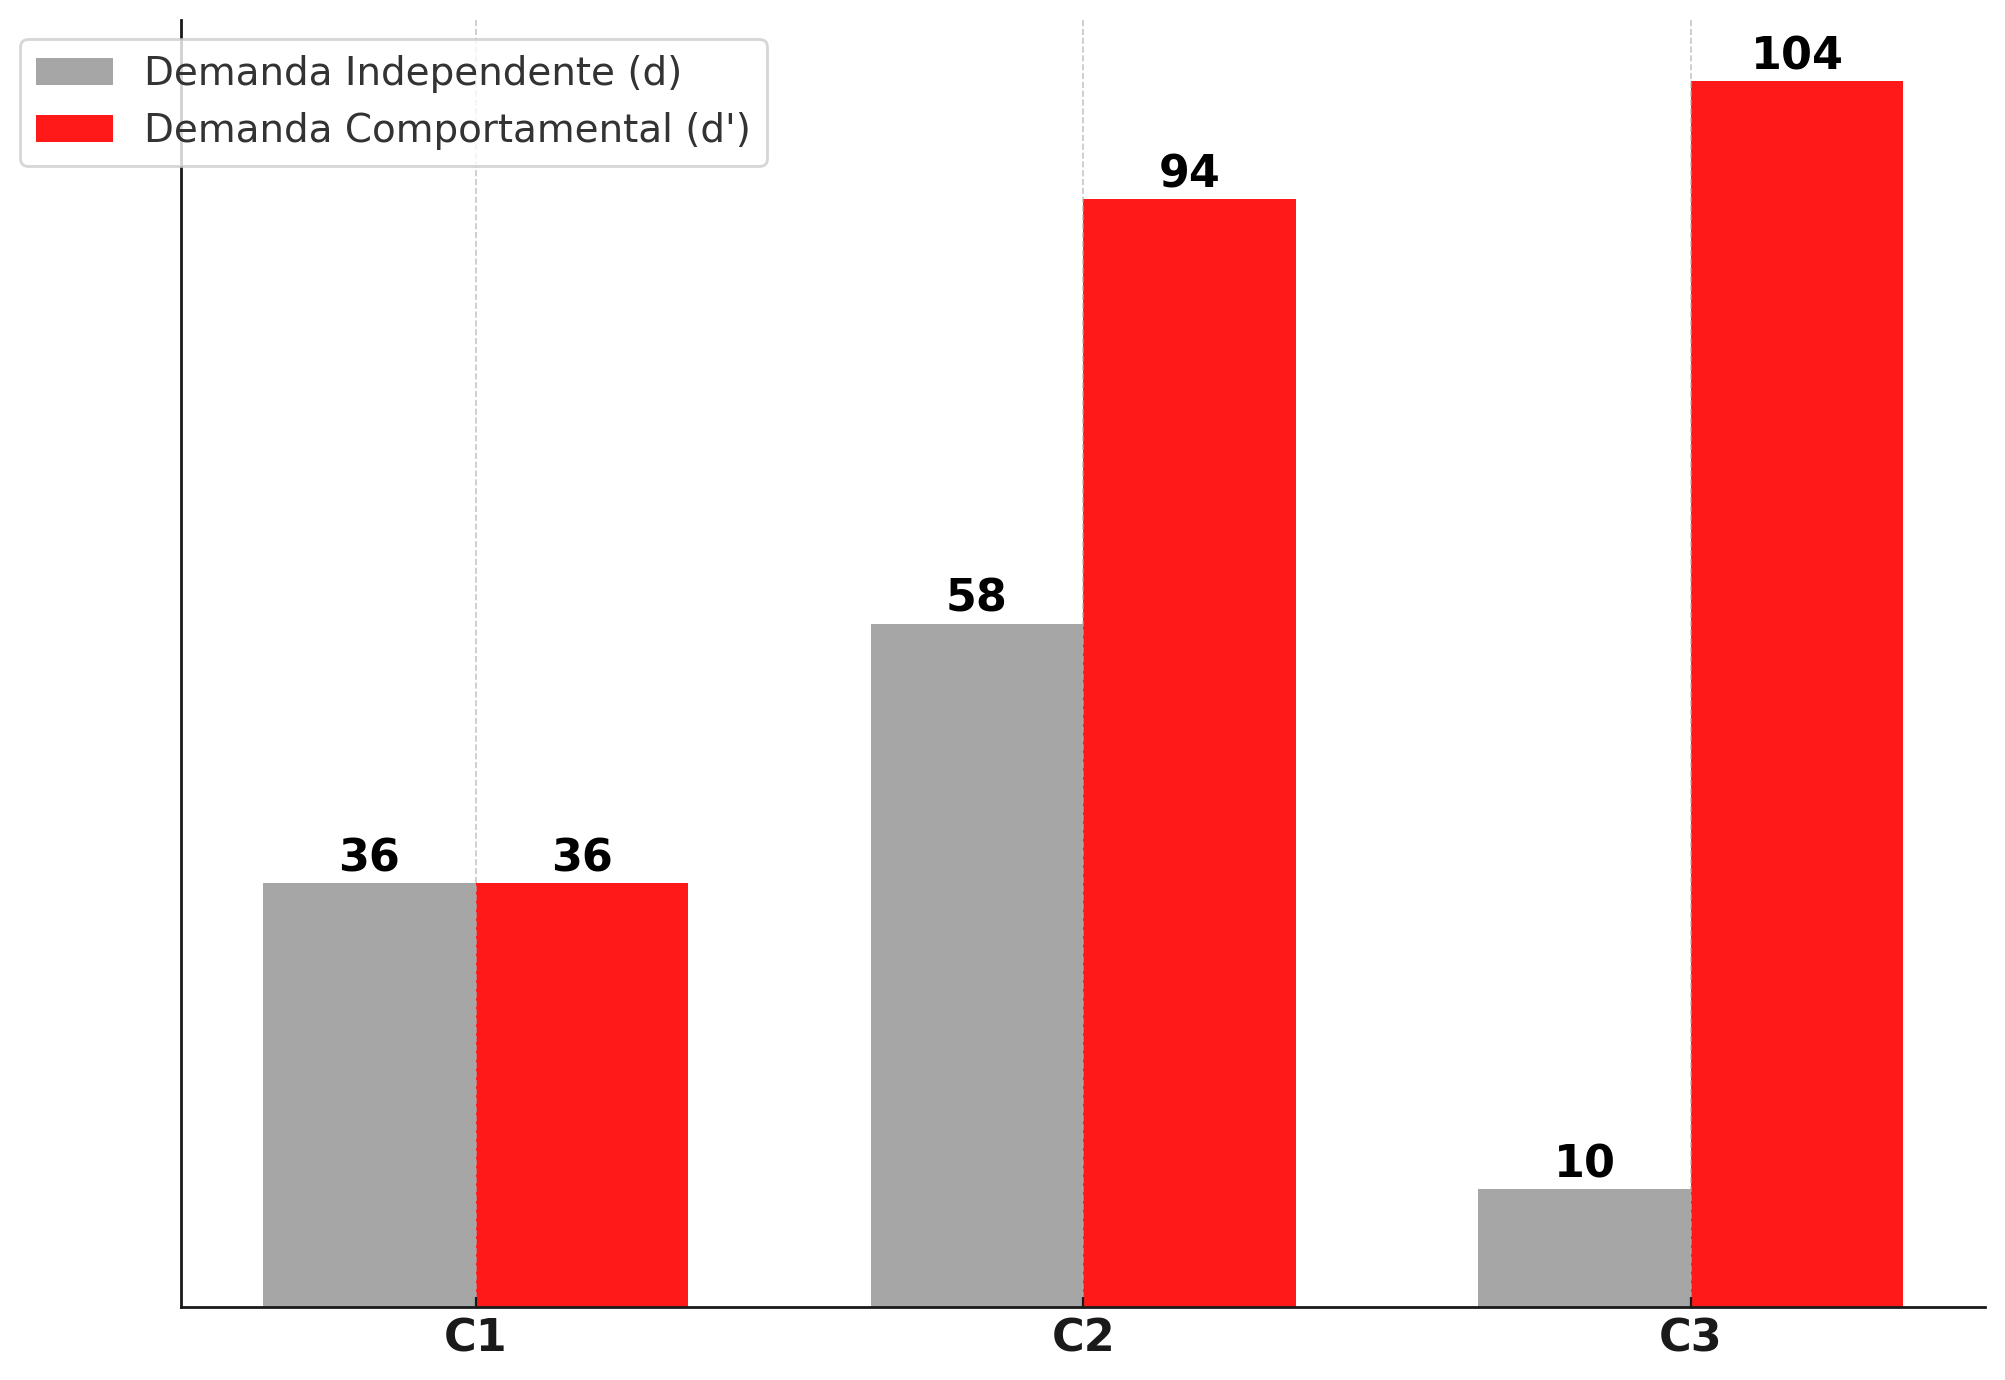
\includegraphics[width=\linewidth]{img/dem_classes.png}
		\caption{Distribuição das Demandas}
		\label{fig:dem_classes}
	\end{subfigure}\hspace{5mm}
	\begin{subfigure}[b]{0.45\linewidth}
		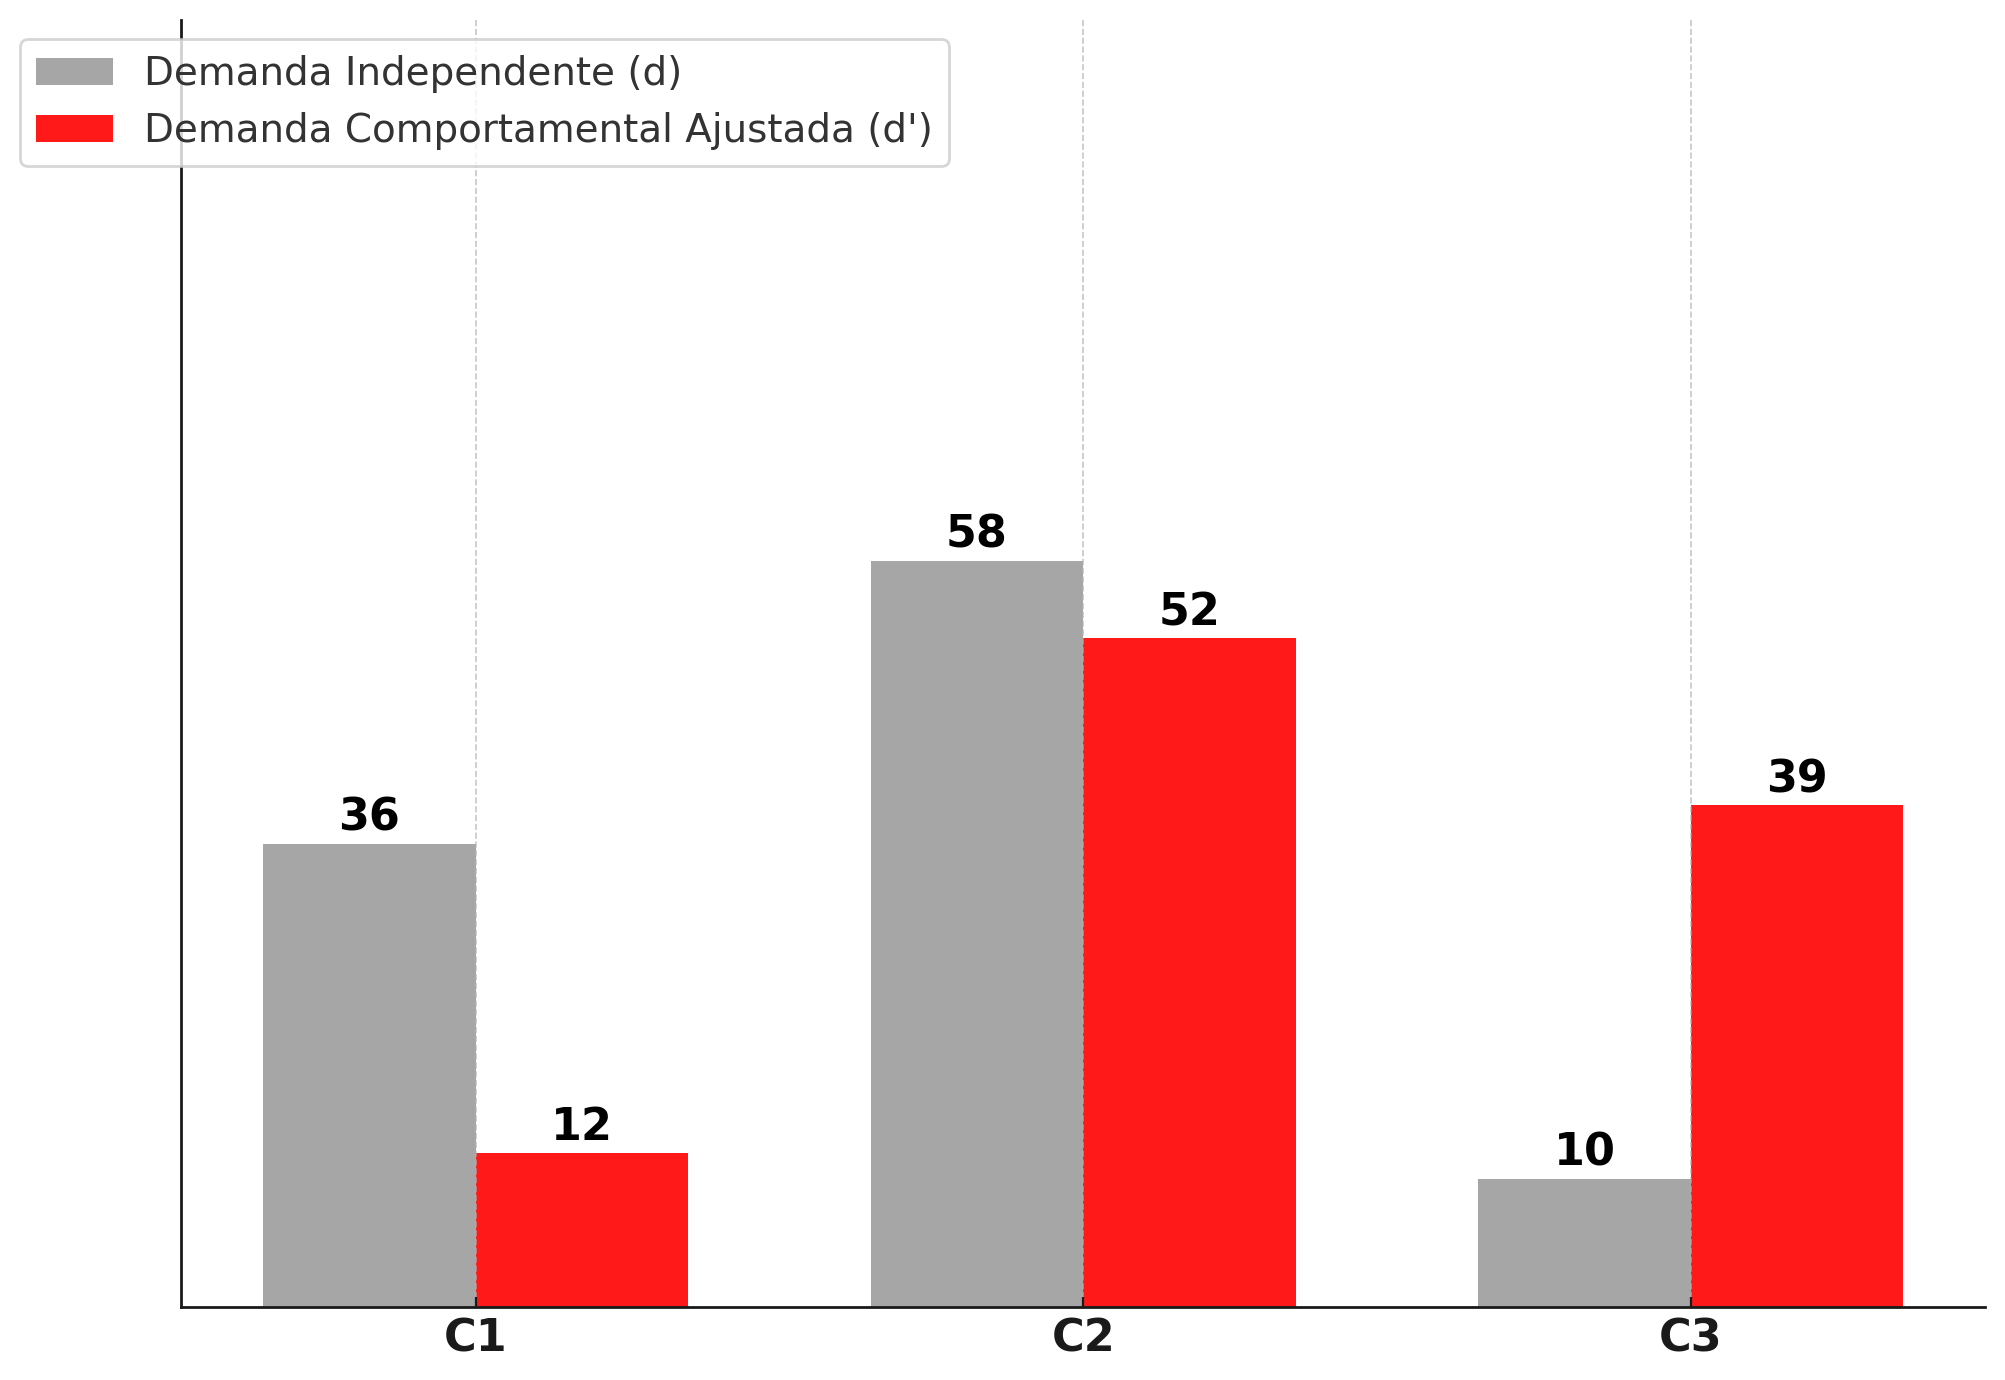
\includegraphics[width=\linewidth]{img/dem_redistri.png}
		\caption{Demanda Comportamental Ajustada}
		\label{fig:dem_redistri}
	\end{subfigure}
	\caption{Ajuste da Demanda Comportamental com Proporções}
	\label{fig: ajustes_demanda}
\end{figure}

O gráfico \ref{fig: ajustes_demanda} nos ajuda a ter uma visão mais clara do problema. Observe que, na parte \ref{fig:dem_classes}, temos a comparação entre a demanda independente $d$ e a demanda comportamental $d'$. Note que, em todos os casos, $d' \geq d$. Independentemente dos valores que $d'$ possa assumir, o modelo selecionará os valores de $d$, pois estes são os que geram o maior lucro.

Após a aplicação do nosso ajuste, na parte \ref{fig:dem_redistri}, observe como "reduzimos a demanda" \, tanto da classe $c_1$ quanto da classe $c_2$ para redistribuí-la à classe $c_3$. Agora, $d'$ não é sempre maior ou igual a $d$, e o modelo é forçado a considerar o limite inferior, o que resulta na inclusão da demanda comportamental ajustada.

Em outras palavras, isso reflete uma situação em que parte das pessoas que estavam dispostas a pagar mais caro chegaram primeiro, mas encontraram opções mais baratas disponíveis e aproveitaram essa situação para realizar suas compras. Esse ajuste garante que o modelo capture um comportamento de compra mais realista e alinhado à flexibilidade das preferências dos clientes.

Outra abordagem proposta, como alternativa às restrições \ref{eq: m2_dem_compor_porcentaje_dem} e \ref{eq: m2_dem_compor_porcentaje_dem_last}, foi o controle da demanda, desta vez criando uma hierarquia descendente para as classes da variável de decisão $X$, considerando um determinado tipo de assento, trecho e período. Em teoria, essa estratégia homogeneiza os valores que $X$ poderia assumir, atribuindo valores muito semelhantes a todas as classes dentro das condições especificadas. Vejamos a restrição e um exemplo:

\allowdisplaybreaks
\begin{align}
	&X_{ijvkt} \leq X_{i,j,v,k+1,t}, \quad   \forall(i,j) \in OD, v \in V, k \in K_v / k \neq max\{K_v\}, t \in T  \label{eq: m2_ajuste_hierarquia}
\end{align}

Retomemos novamente o exemplo apresentado na Tabela \ref{tab: exemplo_ajuste_demanda}. Se aplicarmos essa nova lógica, o resultado esperado seria que $X_{\textcolor[rgb]{0.0588, 0.5412, 0.4275}{c_1}} \leq X_{\textcolor[rgb]{0.0588, 0.5412, 0.4275}{c_2}} \leq X_{\textcolor[rgb]{0.0588, 0.5412, 0.4275}{c_3}}$. No entanto, como neste ponto (antes de adicionar as restrições que complementam a demanda comportamental) o modelo ainda se comporta como independente — uma situação já explicada anteriormente —, o modelo utilizaria a demanda independente como base para criar a hierarquia descendente. É importante destacar algo crucial: mencionamos que o modelo considera a demanda independente para ajustar a hierarquia. No entanto, ao formular a restrição, utilizamos a variável $X$ e não o parâmetro $d'$. Isso não é uma contradição e foi feito intencionalmente. Na verdade, essa escolha foi realizada para explicar, de forma prática, como o modelo funciona internamente. Dito isso, uma solução para o nosso exemplo seria:

\begin{figure}[H]
	\centering
	\begin{subfigure}[b]{0.45\linewidth}
		\centering
		\begin{tabular}{lcccc}
			\toprule
			\textbf{} & \textbf{Classes} & \textbf{$d$} & \textbf{$d'$} & \textbf{X} \\
			\midrule
			& $c_1$ & 36  & 36  & \textbf{34} \\
			& $c_2$ & 58  & 94  & \textbf{35} \\
			& $c_3$ & 10  & 104 & \textbf{35} \\
			\midrule
			& \textbf{Total} & 104 & & \\
			\bottomrule
		\end{tabular}
		\caption{Exemplo restrição  \ref{eq: m2_ajuste_hierarquia}}
		\label{tab:exe_ajuste_dem_hierarquia}
	\end{subfigure}\hspace{5mm}
	\begin{subfigure}[b]{0.45\linewidth}
		\centering
		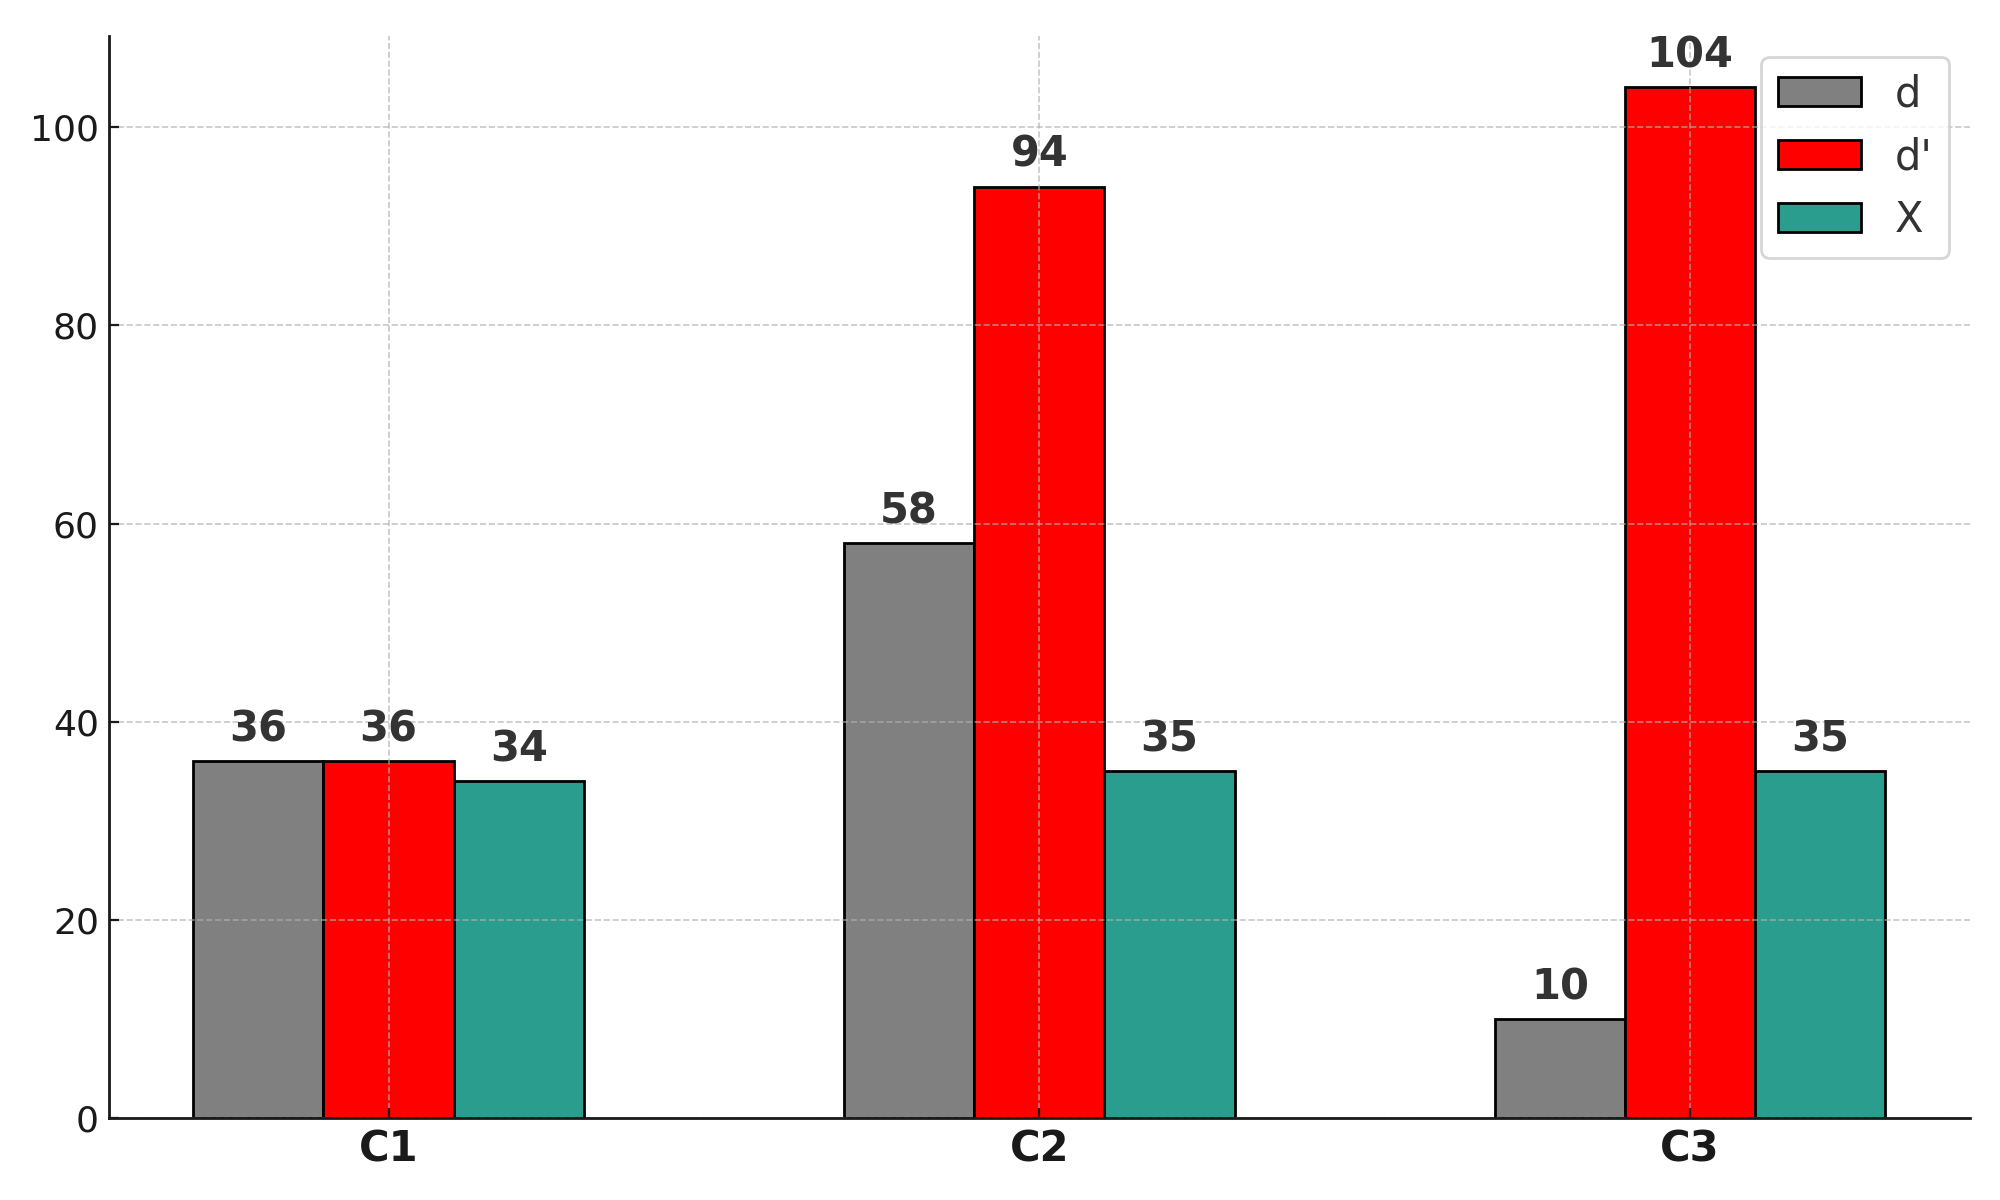
\includegraphics[width=\linewidth]{img/dem_hierar.png}
		\caption{Exemplo visual da restrição \ref{eq: m2_ajuste_hierarquia}}
		\label{fig:dem_classes}
	\end{subfigure}
	\caption{Ajuste da Demanda Comportamental com Hierarquia}
	\label{fig:ajustes_demanda_hierar}
\end{figure}

Nesse caso, a coluna $X$ representa a solução mais gulosa que a variável $X$ poderia assumir. Observe como os valores são muito semelhantes para cada classe e respeitam a ordem decrescente.

Esse último enfoque não requer intervenção direta na demanda comportamental já calculada (assim como o primeiro enfoque). Apenas adicionamos uma condição para a variável $X$, que é suficiente para ativar a característica de lista de preferências do modelo.







































% \section{Segunda modelagem matemática}\label{sec:modelo2}

% Vamos considerar novamente uma versão simplificada do problema. Na verdade, para esta modelagem, serão levadas em conta as mesmas variáveis do primeiro modelo, exceto a variável de disponibilidade \(A\), conforme mostrado a seguir:

% \noindent $x_{ij}$: Quantidade de assentos que será disponibilizada para venda no trecho com origem em $i$ e destino em $j$, onde $j>i$ \\
% \noindent $P_{ij}$: Preço da passagem no trajeto com origem em $i$ e destino em $j$ \\
% \noindent $Q$: Capacidade do trem

% \noindent Assim, a função objetivo e as restrições são como segue:

% $FO: max \quad x_{12}P_{12} + x_{13}P_{13} + x_{14}P_{14} + x_{23}P_{23} + x_{24}P_{24} + x_{34}P_{34}$

% s.a.

% \noindent{\it Restrições para estações de origem}

% Estação 1: $x_{12} + x_{13} + x_{14} \leq Q $ \\
% \indent Estação 2: $x_{23} + x_{24}  \leq  Q $ \\
% \indent Estação 3: $x_{34} \leq Q $

% \noindent{\it Restrições para estações de destino}

% Estação 2: $x_{12} \leq Q $ \\
% \indent Estação 3: $x_{13} + x_{23}  \leq  Q $ \\
% \indent Estação 4: $x_{14} + x_{24} + x_{34} \leq Q $

% Observe que esta formulação é baseada nos modelos de transporte, onde as estações de origem seriam os depósitos e estão restritas por sua capacidade (capacidade do trem), e as estações de destino seriam os destinos e estão restritas, neste caso, pela mesma capacidade do trem e não pela demanda de cada destino.

% Esta formulação garante que sempre será disponibilizada, no máximo, a capacidade do trem tanto para cada saída quanto para cada chegada do trem. Imagine uma solução viável como a mostrada na figura \ref{fig: fig2}.

% \begin{figure}[h]
% 	\begin{center}
% 		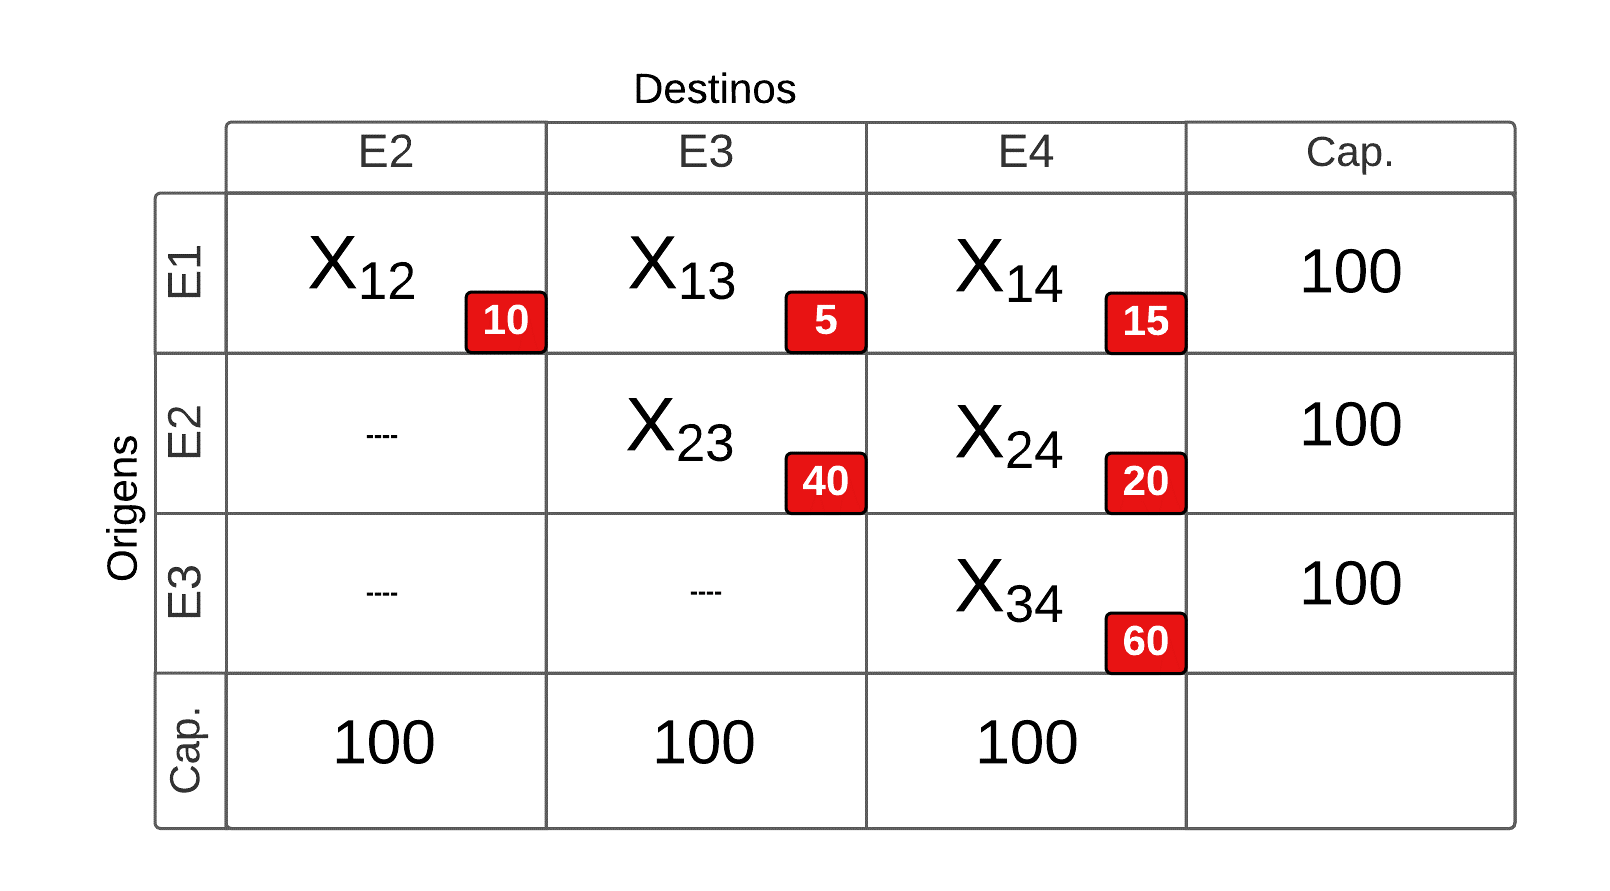
\includegraphics[scale=0.4]{img/fig3.png}
% 		\caption{Solução factível para o problema simplificado}
% 		% Fonte:~\cite{khaksar2013genetic}}
% 		\label{fig: fig3}
% 	\end{center}
% \end{figure}

% Observe que os valores das variáveis são os mesmos que foram mostrados na figura \ref{fig: fig3}. E ainda todas as restrições, tanto por linha quanto por coluna (por origens e por destinos), continuam sendo atendidas.

% \begin{table}[h]
% 	\centering
% 	\small
% 	\begin{tabular}{p{2cm} p{9.5cm} p{3.2cm}}
% 		\toprule
% 		\textbf{Definição} & \textbf{Notação}                                                                                                                                            & \textbf{Domínio}                             \\ \midrule
% 		\multicolumn{3}{l}{\textbf{Conjuntos}}                                                                                                                                                                                          \\ \midrule
% 		$OD$               & Conjunto de Trechos com itinerário                                                                                                                          &                                              \\
% 		$NAD$              & Conjunto de Trechos que NÃO são Adjacentes e que tem itinerário                                                                                             &                                              \\
% 		$BRI_{(o,d)}$      & Conjunto de Trechos contidos dentro de cada trecho $(o,d)$ NÃO Adjacente                                                                                    &                                              \\
% 		$V$                & Conjunto de tipo de assento do trem                                                                                                                                 &                                              \\
% 		$K_v$              & Conjunto de Classes de Control de cada tipo de assento em $V$                                                                                                        &                                              \\
% 		$T$                & Conjunto de Check-Points (Períodos)                                                                                                                         &                                              \\ \midrule
% 		\multicolumn{3}{l}{\textbf{Parâmetros}}                                                                                                                                                                                         \\ \midrule
% 		$Q$                & Capacidade física do trem                                                                                                                                          &                                              \\
% 		$P_{ijvk}$         & Preços  das passagem no Trecho $(i,j)$, tipo de assento $v$ e Classe de Control $k$                                                                                  & $(i,j) \in OD,v \in V, k \in K_v$            \\
% 		$D_{ijvkt}$        & Demanda  das passagem no Trecho $(i,j)$, tipo de assento $v$ e Classe de Control $k$                                                                                 & $(i,j) \in OD,v \in V, k \in K_v, t \in T$   \\ \midrule
% 		\multicolumn{3}{l}{\textbf{Variáveis de decisão}}                                                                                                                                                                               \\ \midrule
% 		$X_{ijvkt}$        & Quantidade de passagem reservadas no trecho $(i,j)$, tipo de assento $v$ e com classe de control $k$ no período $t$                                                  & $(i,j) \in OD, v \in V, k \in K_v, t \in T$  \\
% 		$Y_{ijvkt}$        & Quantidade de passagem autorizados no trecho $(i,j)$, tipo de assento $v$ e com classe de control $k$ no período $t$                                                 & $(i,j) \in OD, v \in V, k \in K_v, t \in T$  \\
% 		$\gamma_{ijvkt}$      & É uma variável binaria que toma o valor de 1 quando $Y_{ijvkt} \neq 0$ e toma  valor de 0 caso contrario, aplica-se apenas a trechos que não são adjacentes & $(i,j) \in NAD, v \in V, k \in K_v, t \in T$ \\
% 		\bottomrule
% 	\end{tabular}
% 	\caption{Notação matemática do problema}
% 	\label{tab: m2_definicao}
% \end{table}
% \begin{align}
% 	 & Max \quad Z = \sum_{(i,j)\in OD} \sum_{v\in V} \sum_{k\in K_v} \sum_{t\in T} P_{ijvk} X_{ijvkt}                                 \label{eq: m2_fo}                          \\
% 	 & \text{s.a.}  \notag                                                                                                                                                        \\
% 	 & \sum_{(i,j)\in OD}\sum_{v\in V}\sum_{k\in K_v}\sum_{t\in T}X_{ijvkt} \leq Q , \quad \forall j / j>1, i<j                        \label{eq: m2_cap_assig_destino}           \\
% 	 & \sum_{(i,j)\in OD}\sum_{v\in V}\sum_{k\in K_v}\sum_{t\in T}X_{ijvkt} \leq Q , \quad \forall i / i<n, j>i                        \label{eq: m2_cap_assig_origem}            \\
% 	 & Y_{ijvkt} \geq Y_{i,j,v,k+1,t},  \quad \forall (i,j),v,k,t / i < j, k < \lVert K_v \rVert,  P_{ijvk} \geq P_{i,j,v,k+1}         \label{eq: m2_jerar_class}                 \\
% 	 & X_{ijvkt} \leq D_{ijvkt},  \quad \forall (i,j),v,k,t/ i < j                                                                     \label{eq: m2_assig_menor_dem}             \\
% 	 & \sum_{(i,j) \in OD}\sum_{v\in V}\sum_{t\in T} Y_{i,j,v,k,t} \leq Q, \quad  k = min\{K_v\}, \forall i \in OD                     \label{eq: m2_cap_autho_1er_class}         \\
% 	 & Y_{i,j,v,k,t} \geq  X_{i,j,v,k,t},  \quad k = max\{K_v\}, \forall(i,j),v,t                                                      \label{eq: m2_autho_mayor_assig_1er_class} \\
% 	 & Y_{i,j,v,k,t} \geq  X_{i,j,v,k,t} + Y_{i,j,v,k + 1,t} , \forall(i,j),v, k, t / k < \lVert K_v\rVert                             \label{eq: m2_autho_mayor_assig_mas_autho} %\\
% 	%  & \gamma_{o,d,v,k,t} \leq Y_{o,d,v,k,t} \leq \gamma_{o,d,v,k,t} Q, \quad  \forall (o,d)\in NAD, v, k, t                                 \label{eq: m2_activ_bin_autho}             \\
% 	%  & \gamma_{o,d,v,k,t} \leq Y_{i,j,v,k,t} \leq \gamma_{o,d,v,k,t} Q, \quad  \forall (o,d)\in NAD, (i,j) \in BRI_{(o,d)}, v,k,t            \label{eq: m2_autho_igualar_trecho_maior}  \\
% 	%  & X_{ijvkt} \in \mathbb{Z}^+                                                                                                      \label{eq: m2_dom_assig}                  %\\
% \end{align}
% \begin{align}
% 	 & \gamma_{o,d,v,k,t} \leq Y_{o,d,v,k,t} \leq \gamma_{o,d,v,k,t} Q, \quad  \forall (o,d)\in NAD, v, k, t                                 \label{eq: m2_activ_bin_autho}            \\
% 	 & \gamma_{o,d,v,k,t} \leq Y_{i,j,v,k,t} \leq \gamma_{o,d,v,k,t} Q, \quad  \forall (o,d)\in NAD, (i,j) \in BRI_{(o,d)}, v,k,t            \label{eq: m2_autho_igualar_trecho_maior} \\
% 	 & X_{ijvkt} \in \mathbb{Z}^+                                                                                                      \label{eq: m2_dom_assig}                  \\
% 	 & Y_{ijvkt} \in \mathbb{Z}^+                                                                                                      \label{eq: m2_dom_autho}                  \\
% 	 & \gamma_{ijvkt} \in \{0,1\}                                                                                                         \label{eq: m2_dom_bin_nadja}
% \end{align}

% Como já foi mencionado, nesta formulação modificamos as restrições que controlam as variáveis reservadas X, ou seja, mudamos as restrições 1 e 2 do primeiro modelo e eliminamos a variável de decisão Ai.

% % \end{adjustwidth}
% %Note que, na definição, não temos mais a variável de decisão de disponibilidade \(A_i\). Neste caso, a equação \ref{eq: m2_fo} representa a função objetivo que esta tentando maximizar a soma do produto entre as quantidades reservadas e os preços das mesmas, ou seja, estamos maximizando a receita em função das quantidades dos assentos que estão reservados.

% %A restrição \ref{eq: m2_cap_assig_destino} garante que a quantidade total de assentos autorizados para cada destino seja a quantidade máxima de assentos do trem para todas as classes e todos os períodos.
% %A restrição \ref{eq: m2_cap_assig_origem} garante que a quantidade de assentos autorizados para cada origem seja no máximo a capacidade do trem para todas as classes e todos os períodos.
% %As restrições de \ref{eq: m2_cap_autho_1er_class} a \ref{eq: m2_dom_autho} representam o mesmo que o primeiro modelo já exposto.\\

% Para este caso, as restrições \ref{eq: m2_cap_assig_destino} e \ref{eq: m2_cap_assig_origem} representam a generalização do problema simplificado, onde a primeira garante que a quantidade de assentos autorizados para venda não viole a capacidade do trem ao chegar a cada estação de destino; e a segunda garante que a quantidade de assentos autorizados respeite a capacidade do trem no momento de sair de cada estação de origem. O restante das restrições foi explicado na formulação 1.